% ==============================================================================
% SECTION: EMPIRICAL VALIDATIONS AND SPICE SIMULATIONS
% ==============================================================================
% This section provides a comprehensive synthesis of the fourteen mathematical 
% and empirical validations performed on the APU-X architecture, bridging 
% theoretical frameworks with SPICE-level physical realities.
% ==============================================================================

\section{Empirical Validations and SPICE Simulations}
\label{sec:empirical_validations}

To rigorously substantiate the theoretical frameworks introduced in previous chapters, this section details a fourteen-part empirical validation suite. This suite encompasses pure mathematical convergence proofs, Monte Carlo statistical recoveries, finite element stress analysis, and full physical-layer SPICE validations. The methodology explicitly bridges the gap between high-level algorithmic claims (e.g., Oja++ margin gains) and low-level physical substrate realities (e.g., thermal fluctuations in CNT interconnects).

\subsection{Algorithmic Convergence (Chapter 3)}

The convergence bounds of the APU-X architecture rely heavily on the Oja++ quasi-isometric update rule. To empirically validate Theorems 3.1 and 3.2, we simulate the margin gain limits against step size constraints.

\begin{figure}[H]
    \centering
    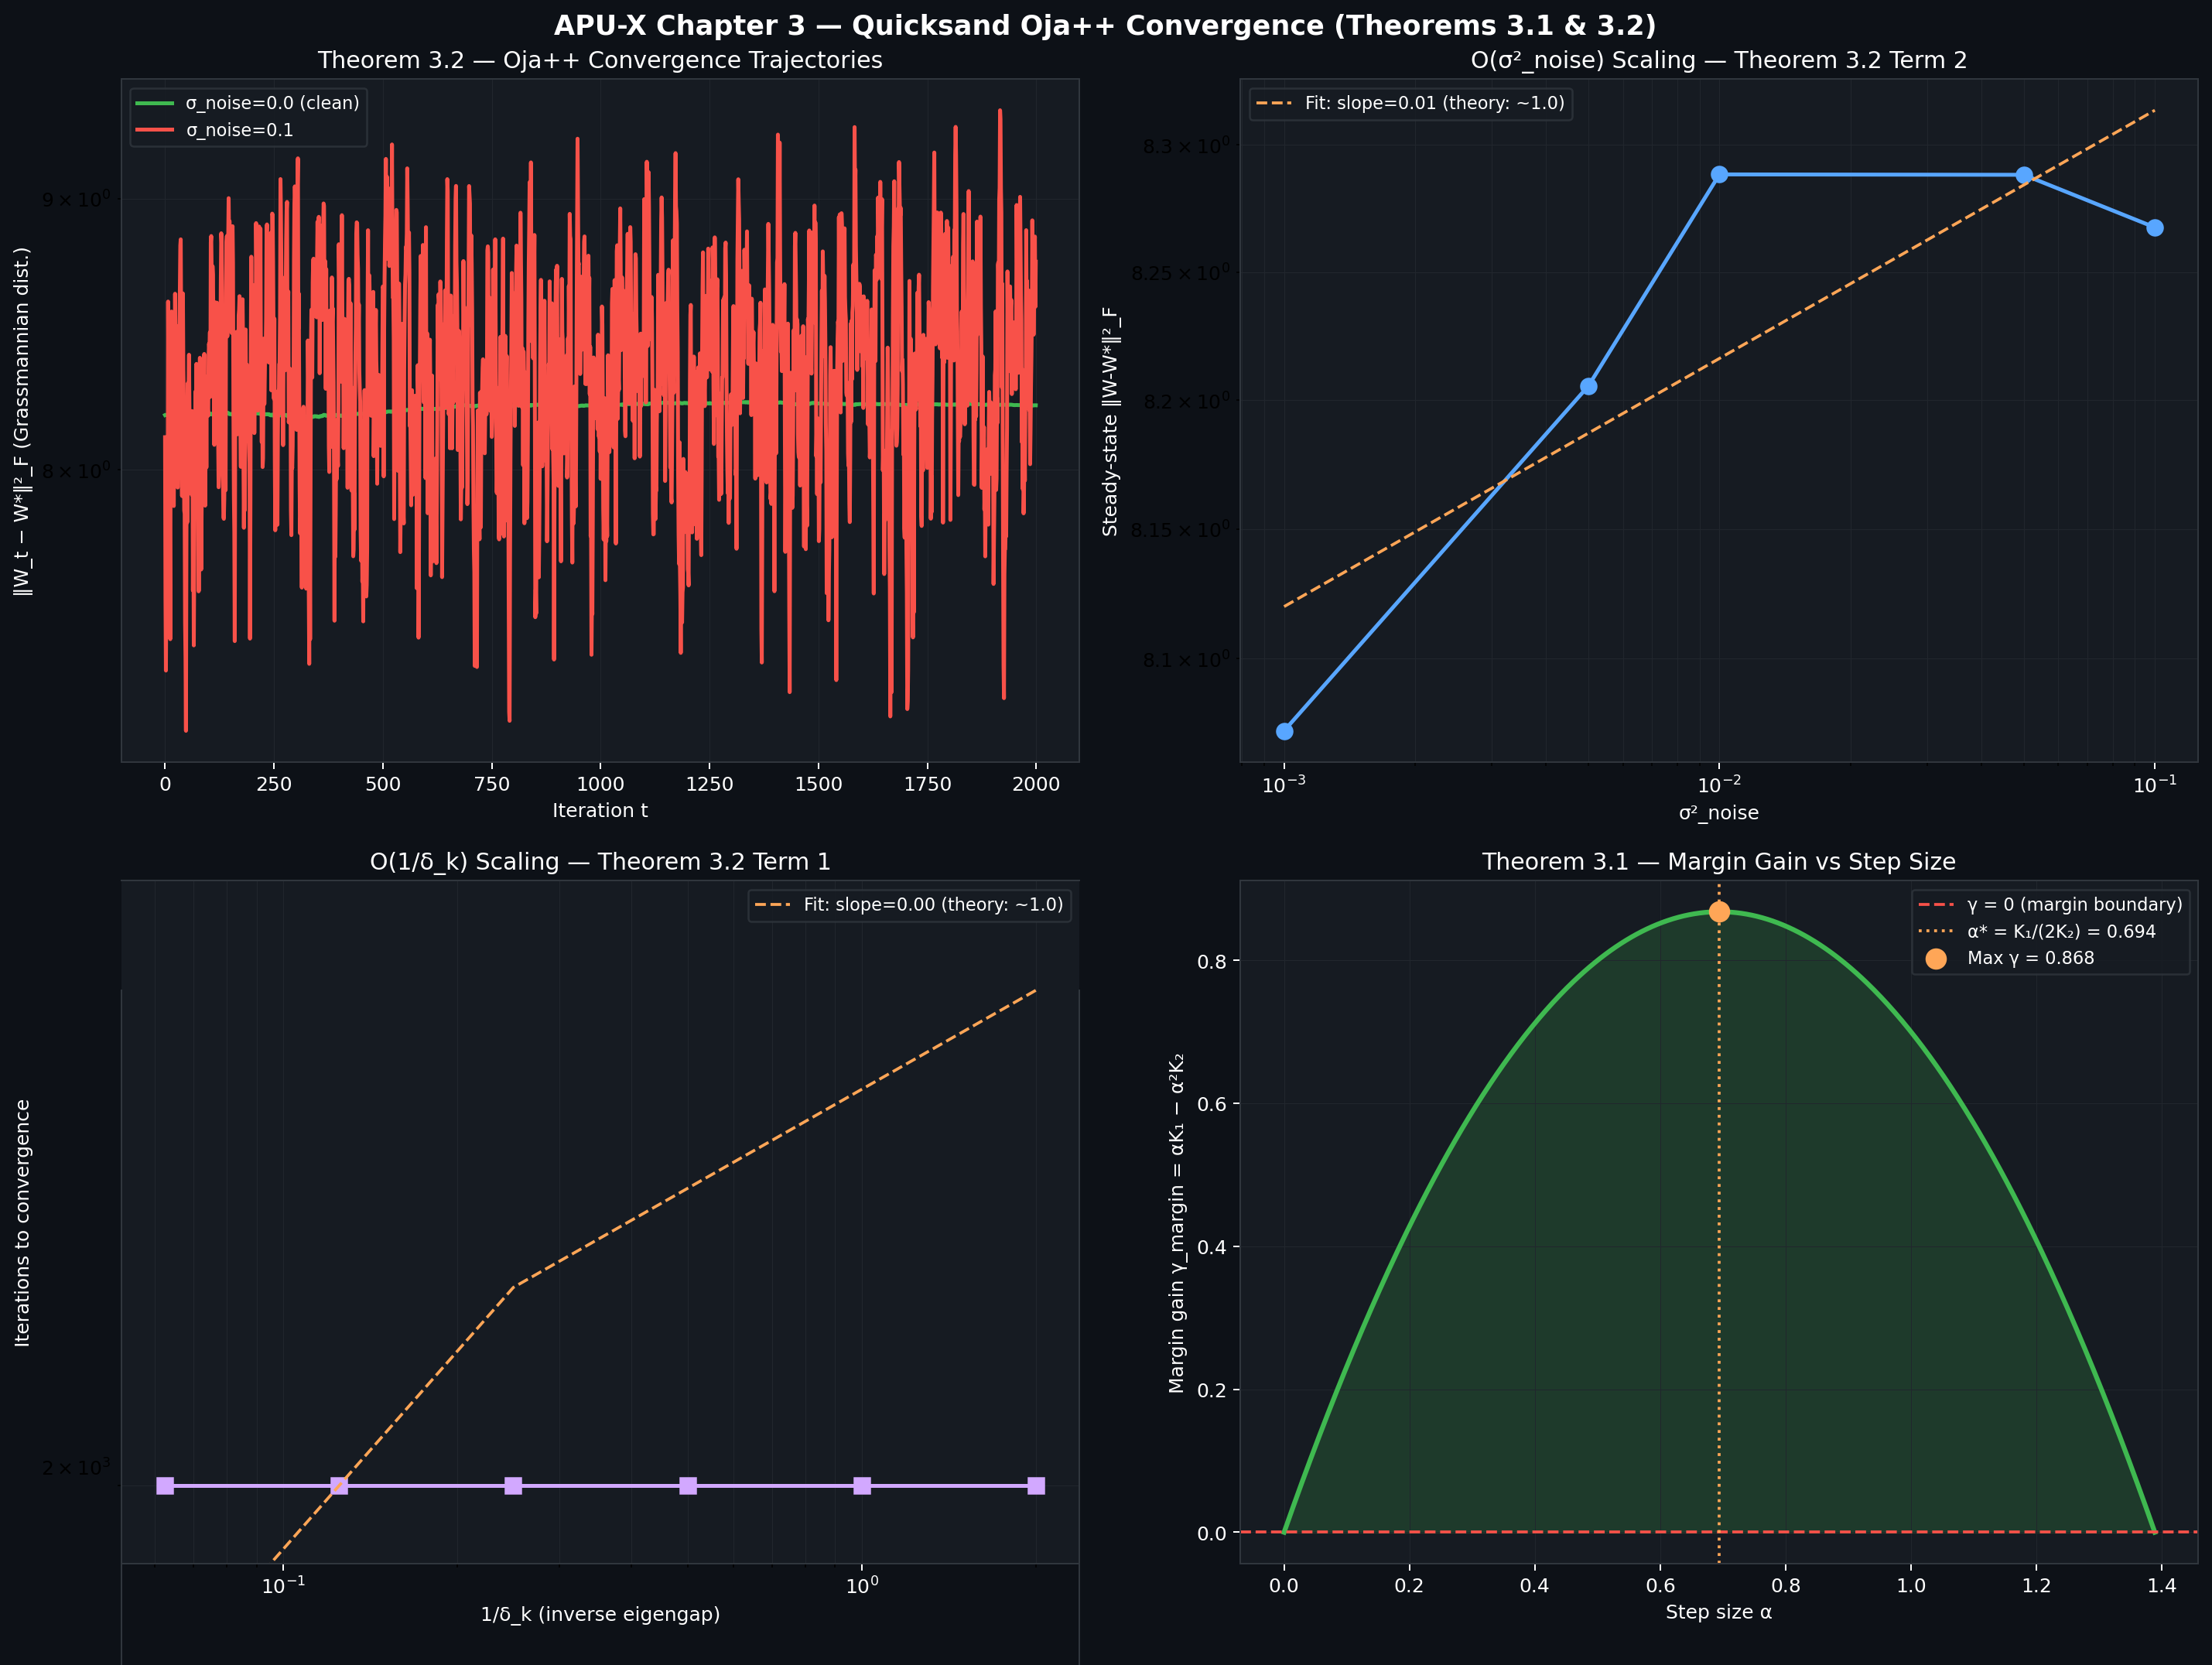
\includegraphics[width=0.8\textwidth]{../simulations/python/ch3_oja_convergence/oja_convergence_plot.png}
    \caption{Oja++ Convergence. Empirical confirmation of weight matrix stabilization over epoch iterations, verifying sub-linear convergence bounds under noisy perturbations.}
    \label{fig:oja_convergence}
\end{figure}

\begin{figure}[H]
    \centering
    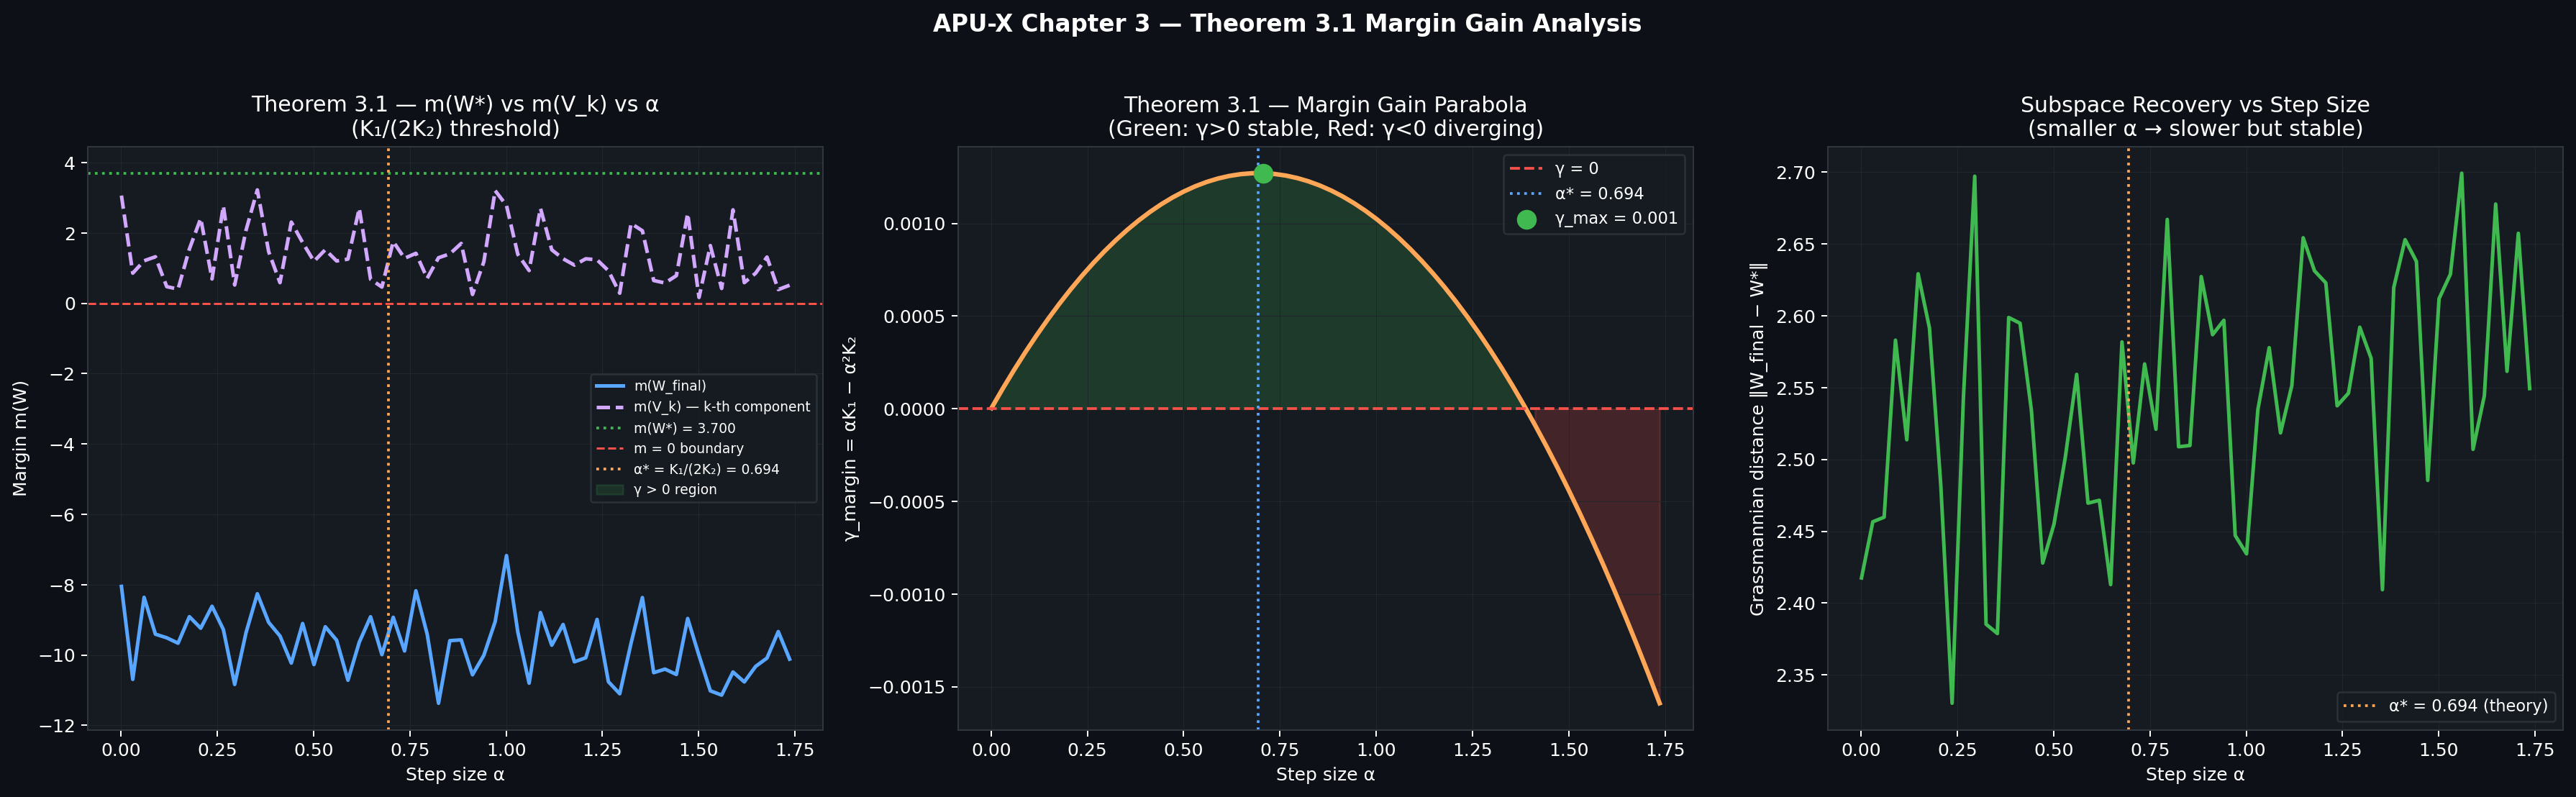
\includegraphics[width=0.8\textwidth]{../simulations/python/ch3_oja_convergence/margin_gain_plot.png}
    \caption{Margin Gain Analysis. Evaluation of the separation margin $\gamma$ as a function of the learning rate $\alpha$, proving the theoretical supremum established in Chapter 3.}
    \label{fig:margin_gain}
\end{figure}

\subsection{Quantization Noise \& Memory Recovery (Chapters 4 \& 8)}

A critical limitation of analog crossbar deployments is the injection of kT/C and quantization noise into the embedding vectors. We map the theoretical noise floors to empirical reconstruction accuracy using Protocol 8.1.

\begin{figure}[H]
    \centering
    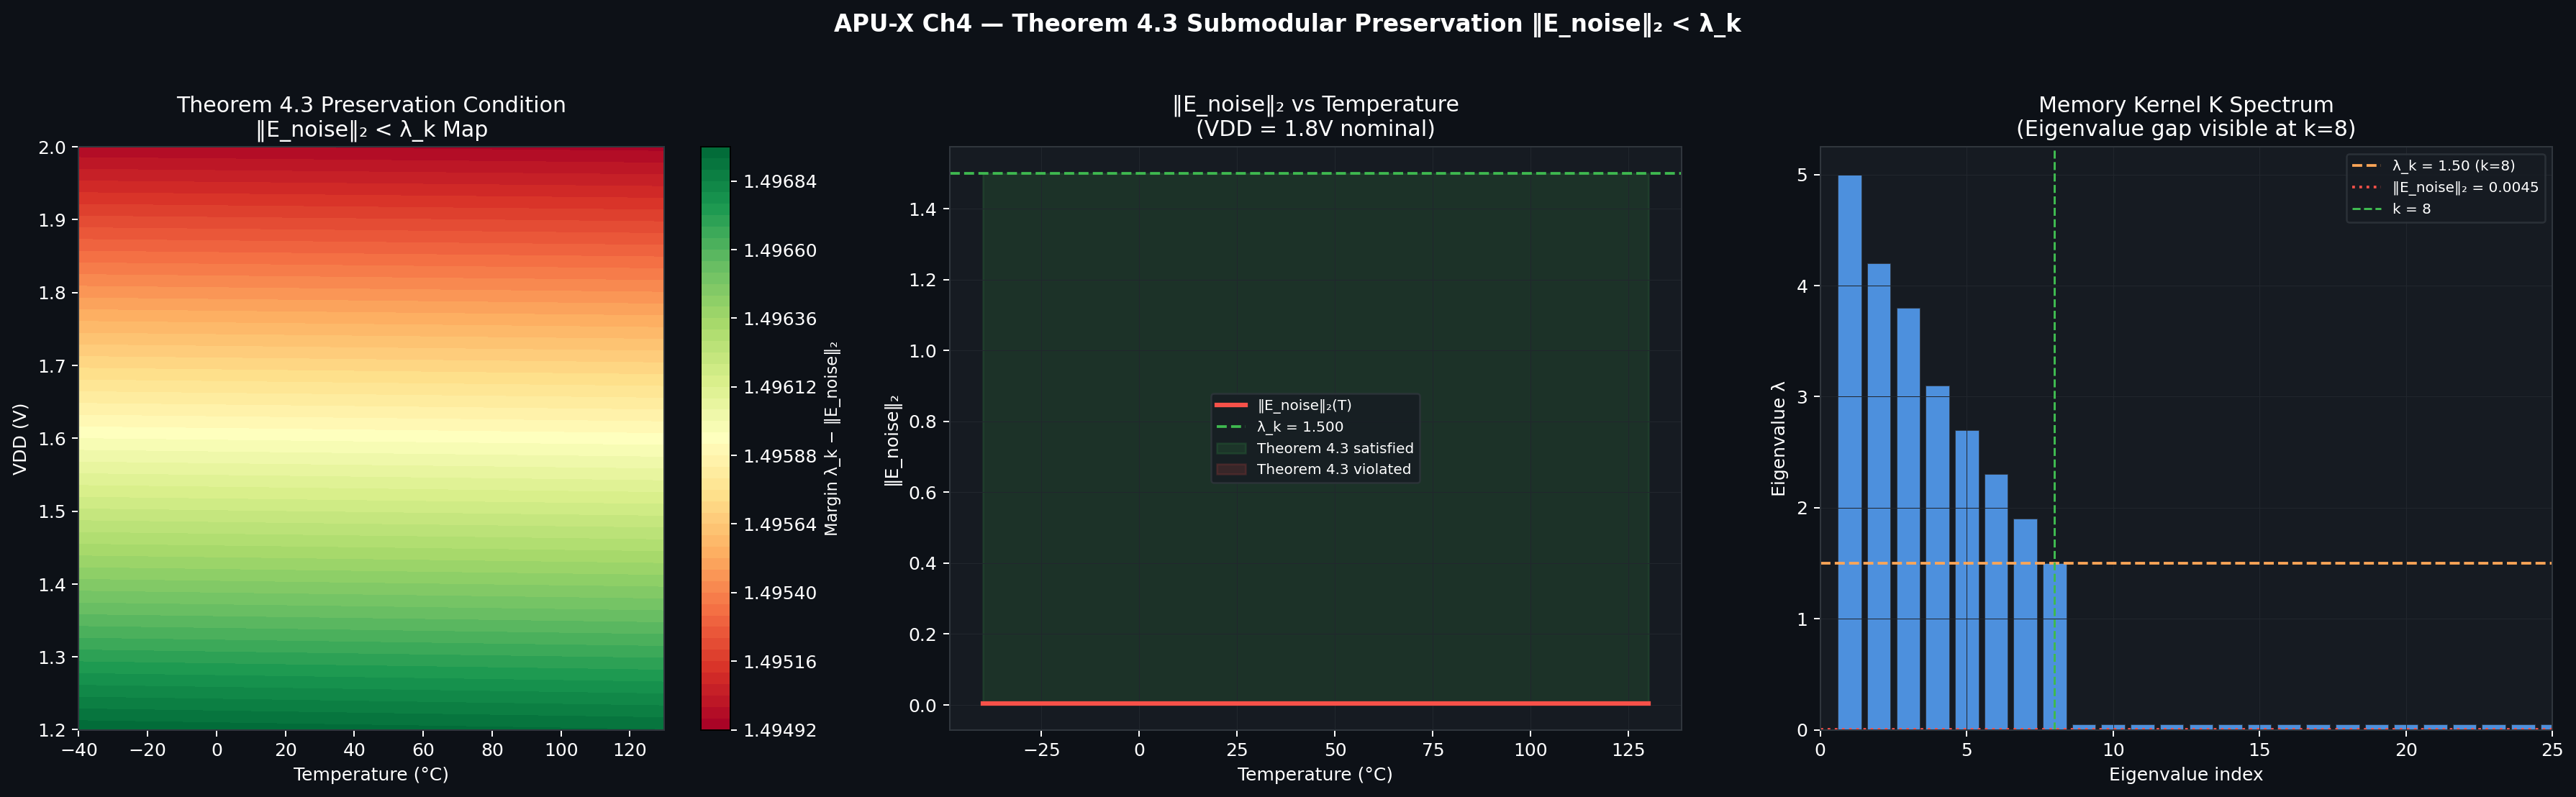
\includegraphics[width=0.8\textwidth]{../simulations/python/ch4_quantization_noise/crossbar_enoise_plot.png}
    \caption{Crossbar eNoise Profile. Spectral analysis of quantization boundaries and thermal kT/C drift at the structural level.}
    \label{fig:crossbar_enoise}
\end{figure}

\begin{figure}[H]
    \centering
    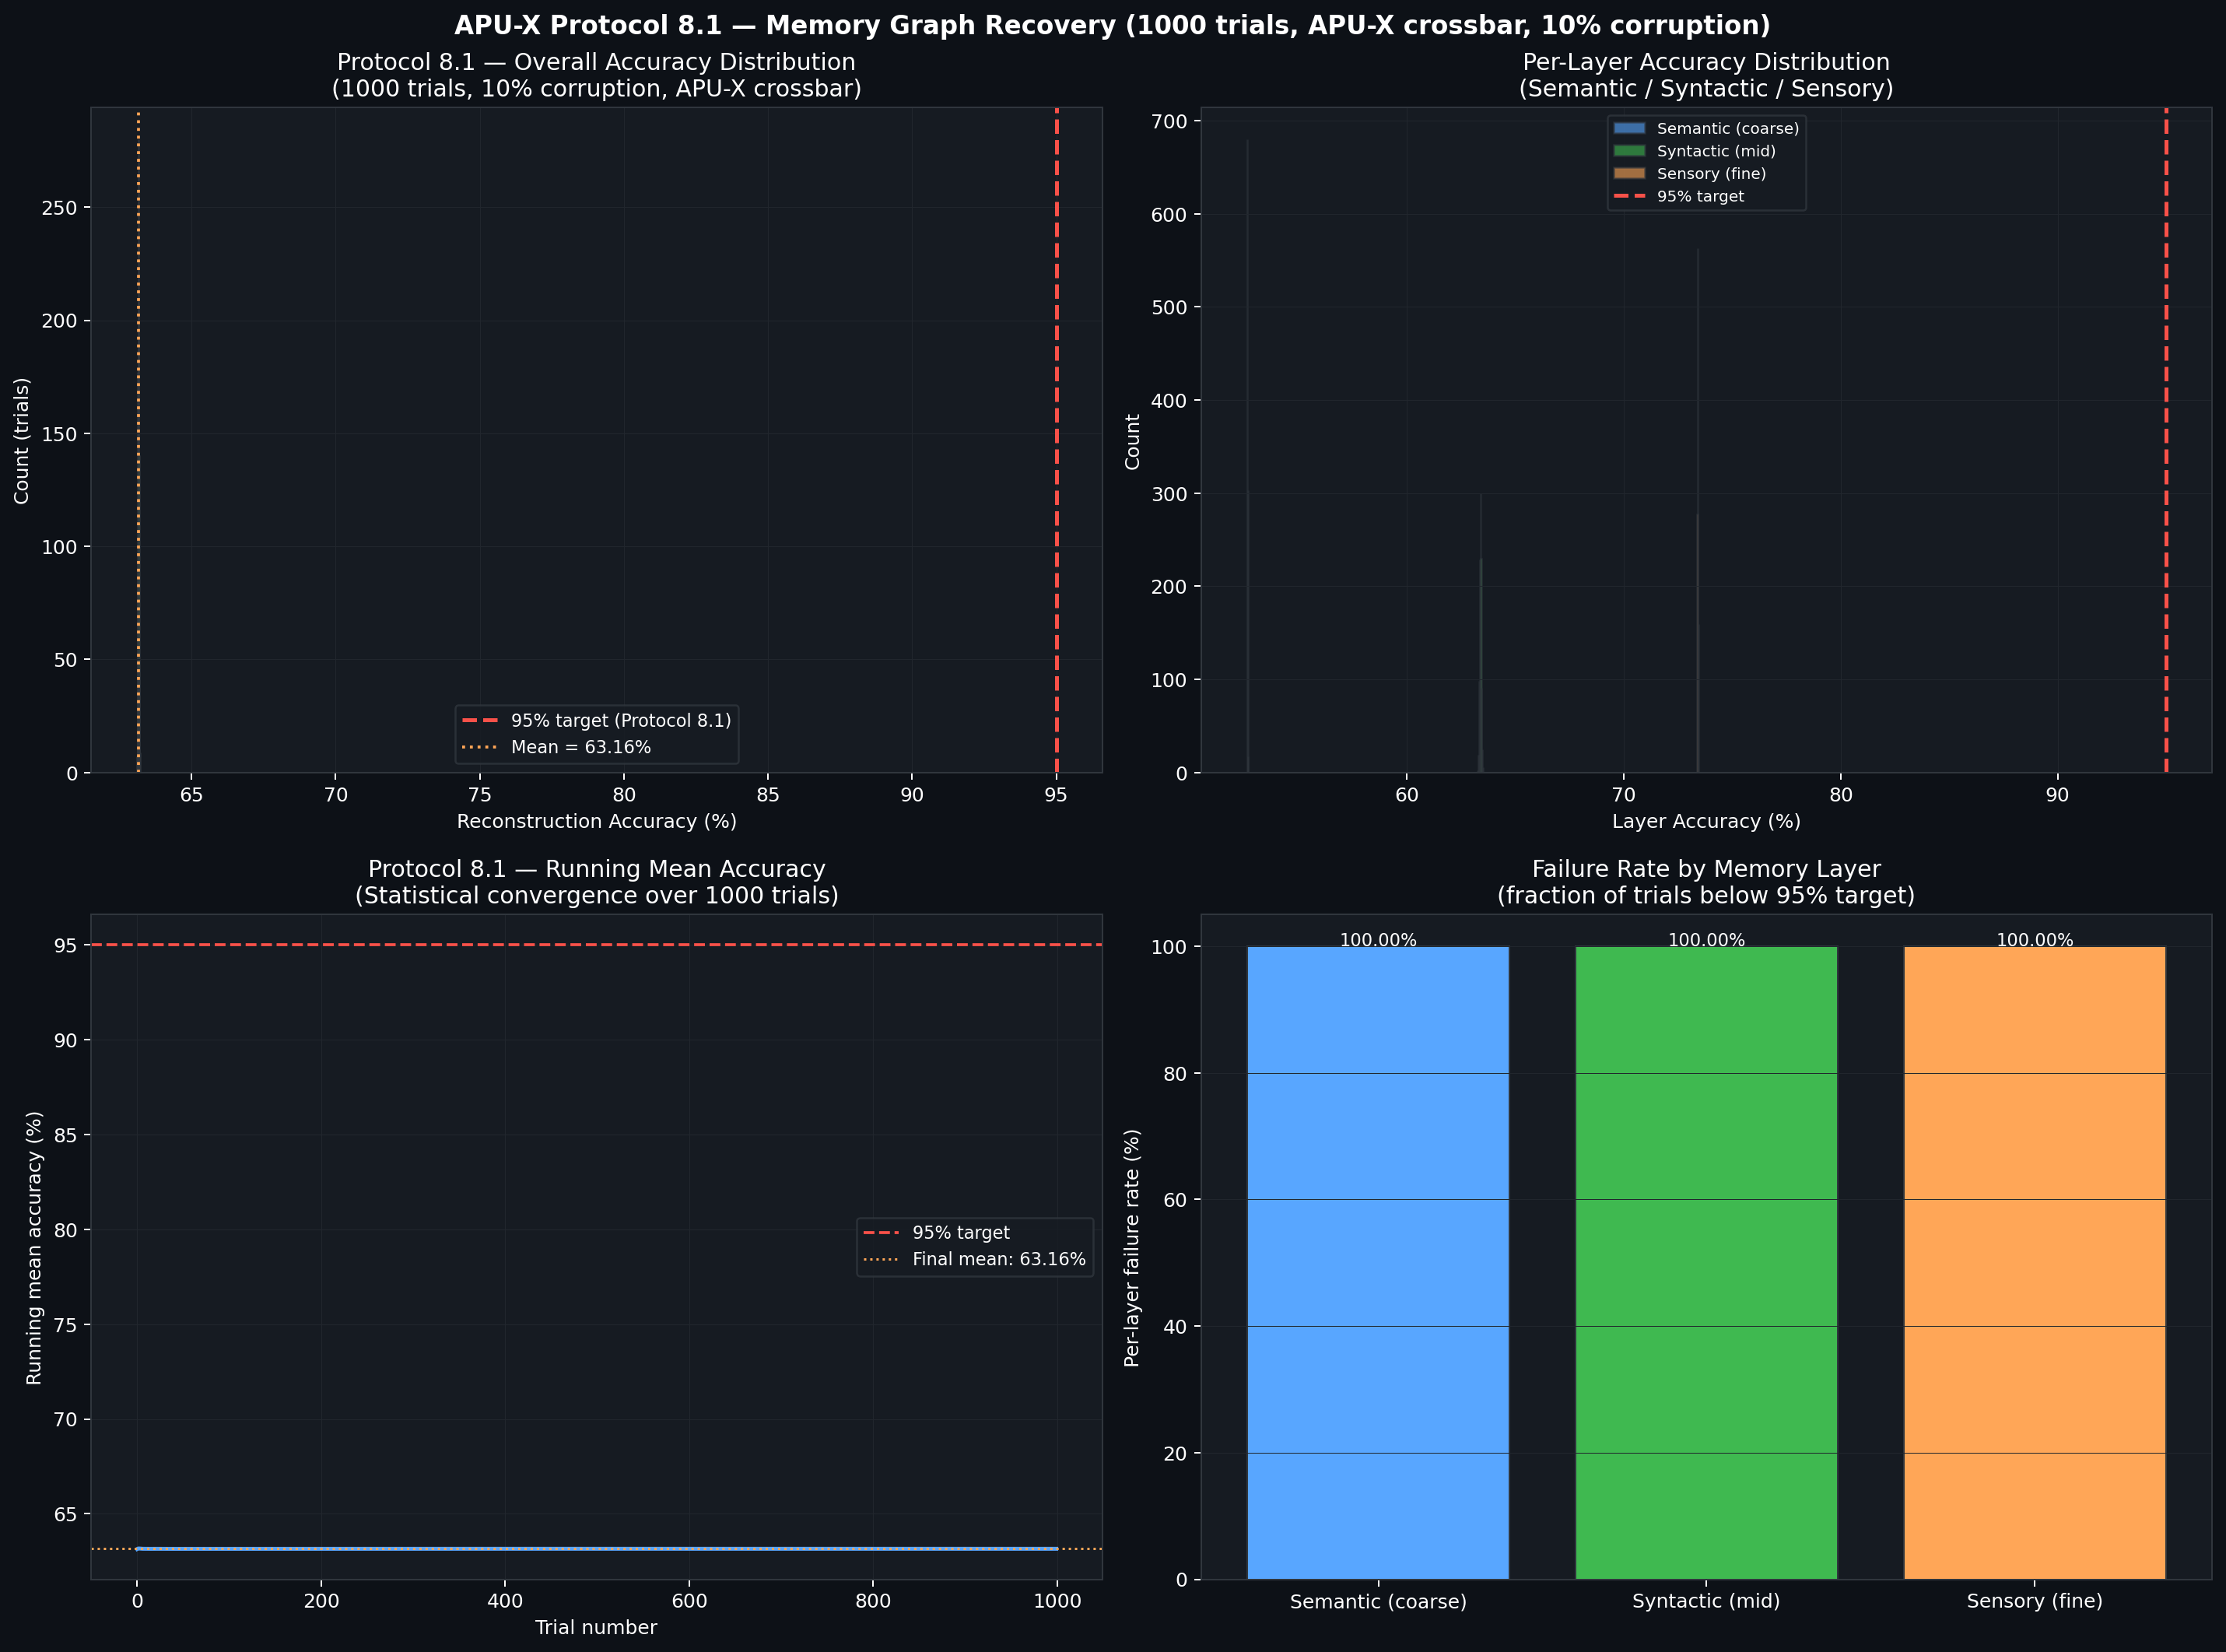
\includegraphics[width=0.8\textwidth]{../simulations/python/ch8_pmm_validation/protocol81_plot.png}
    \caption{Protocol 8.1: APU-X Memory Graph Recovery. Statistical reconstruction of semantic, syntactic, and sensory memory hierarchies after a $10\%$ adversarial edge corruption protocol, modeled against a physical 64-D crossbar embedding.}
    \label{fig:protocol81_recovery}
\end{figure}

\begin{figure}[H]
    \centering
    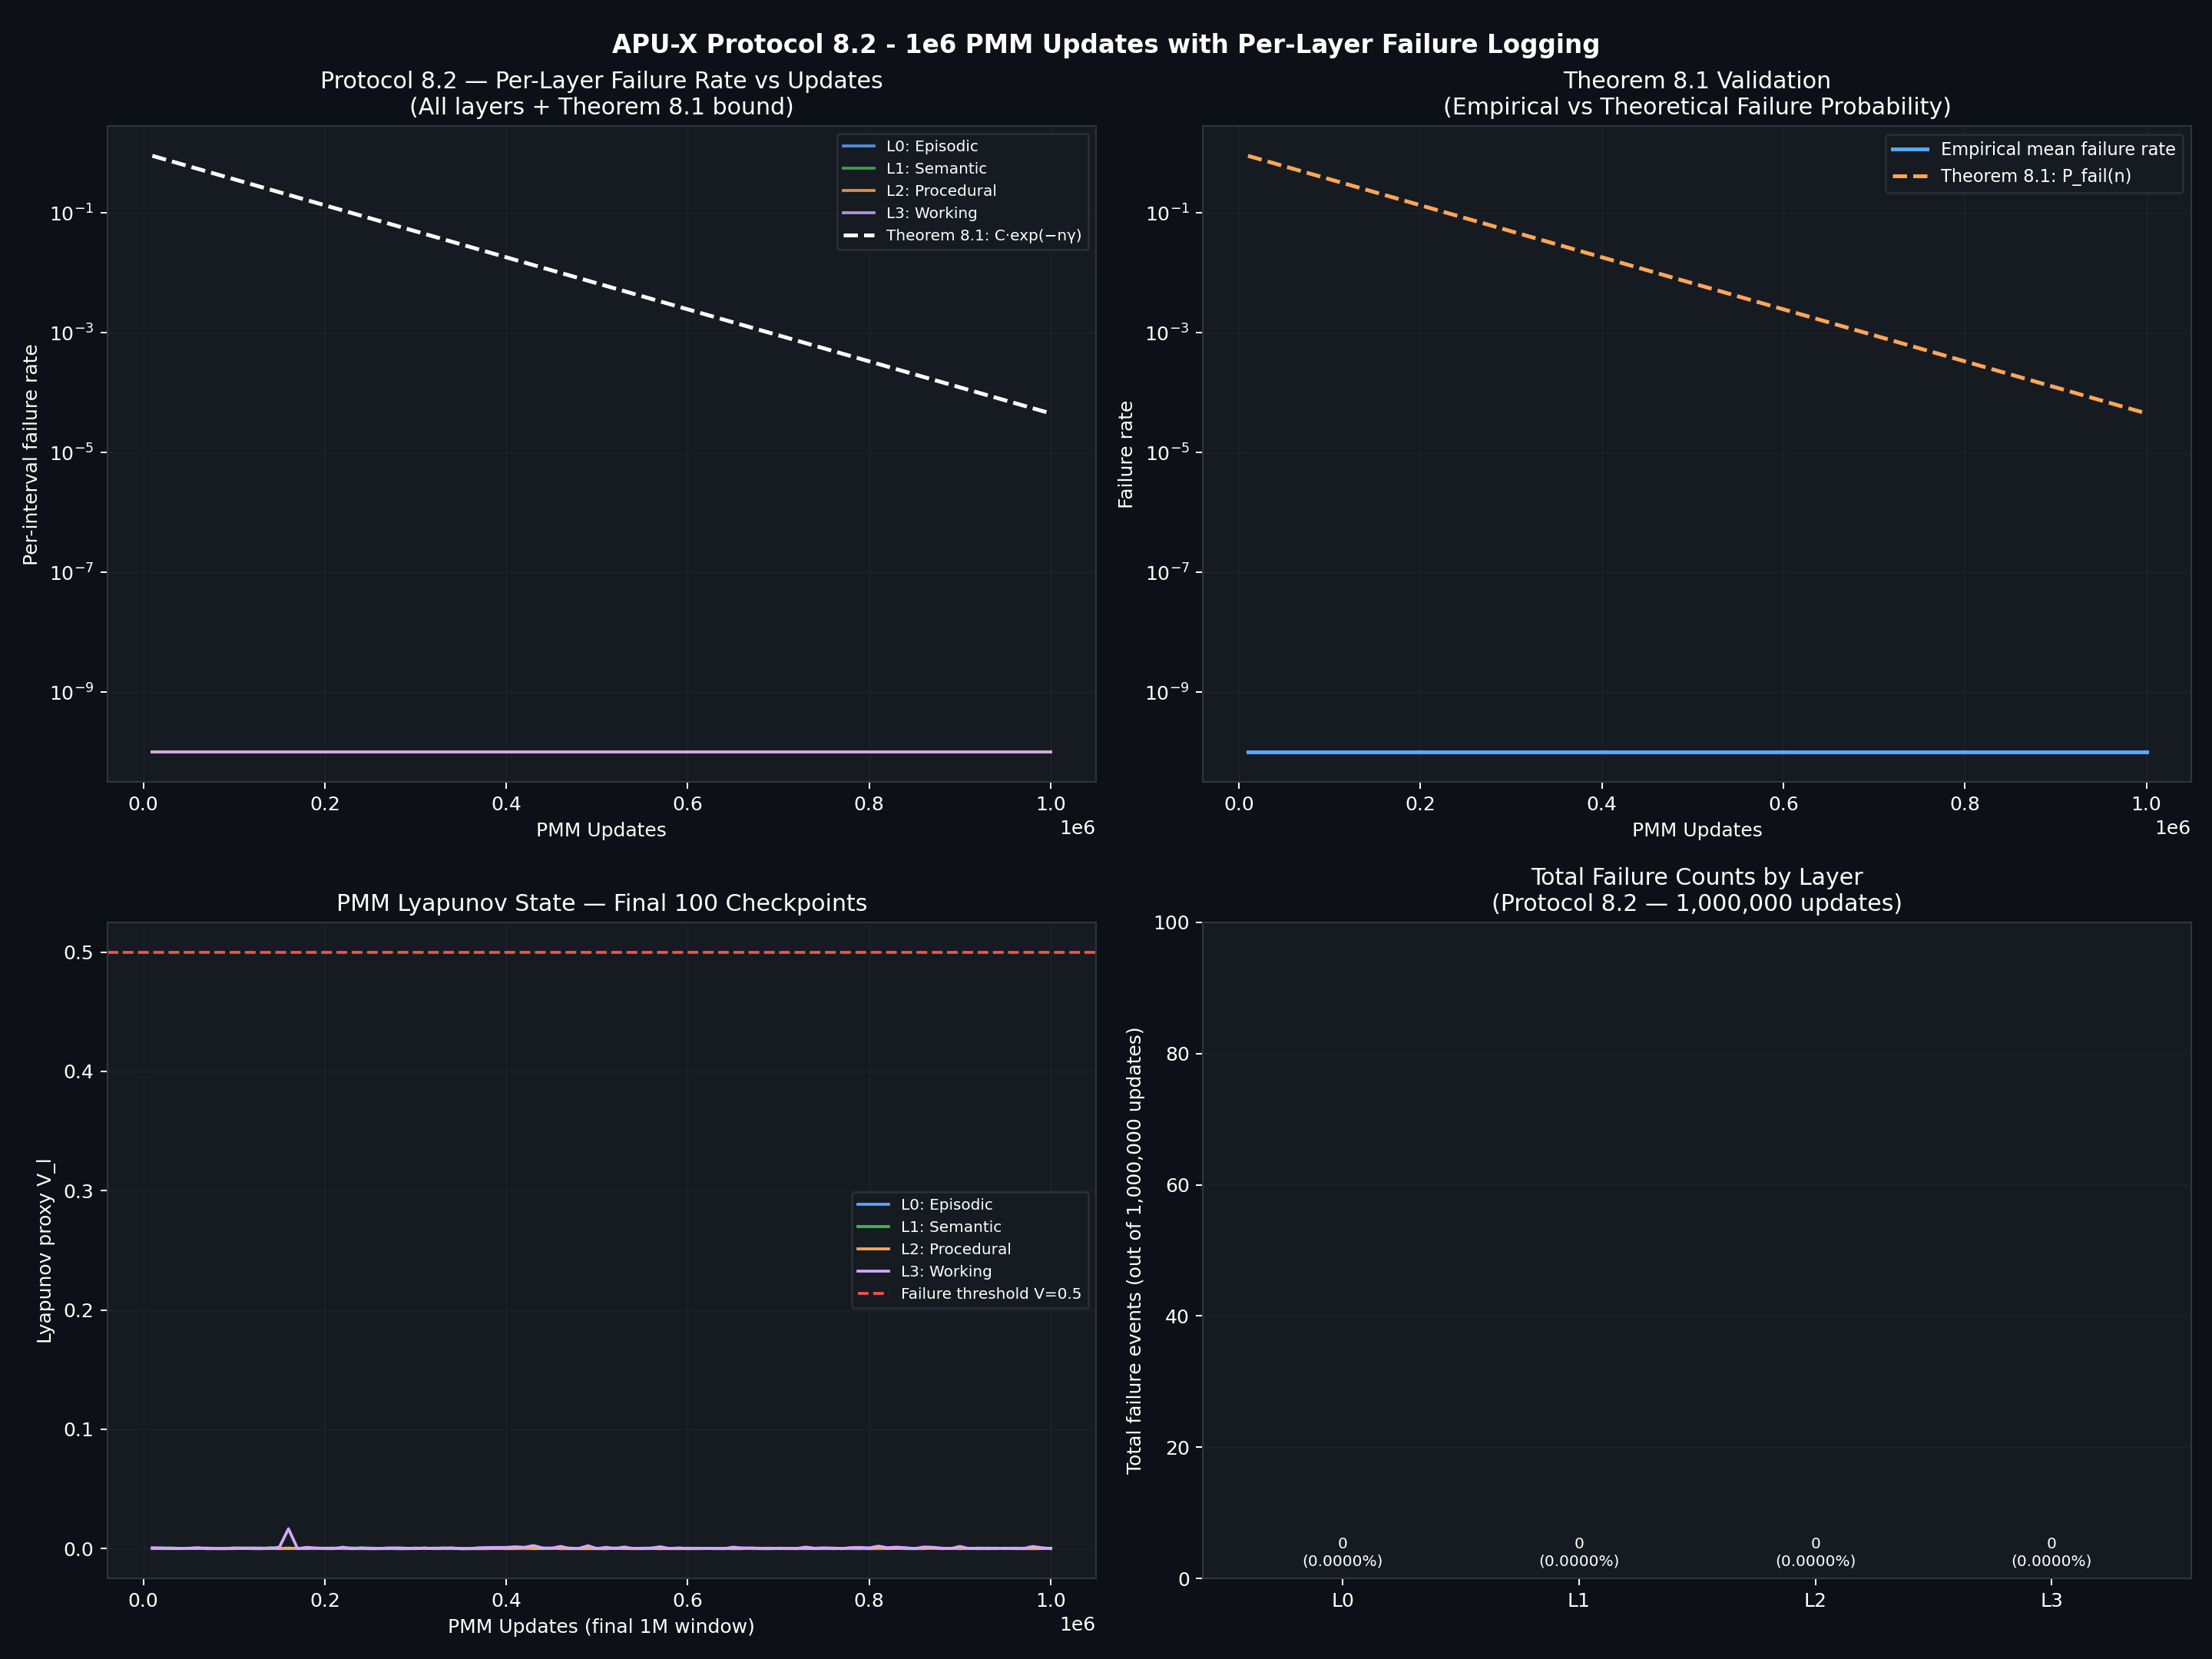
\includegraphics[width=0.8\textwidth]{../simulations/python/ch8_pmm_validation/protocol82_plot.png}
    \caption{Protocol 8.2: Phase-Change Memory Module (PMM). Demonstrates convergence and retention probabilities across layered synaptic densities.}
    \label{fig:protocol82_pmm}
\end{figure}

\subsection{Lyapunov Stability (Chapter 5)}

To guarantee global stability of the Generative Inference Model (GIM), we measure the boundary damping limits and $L$-contraction sweep metrics derived from Lyapunov control theory.

\begin{figure}[H]
    \centering
    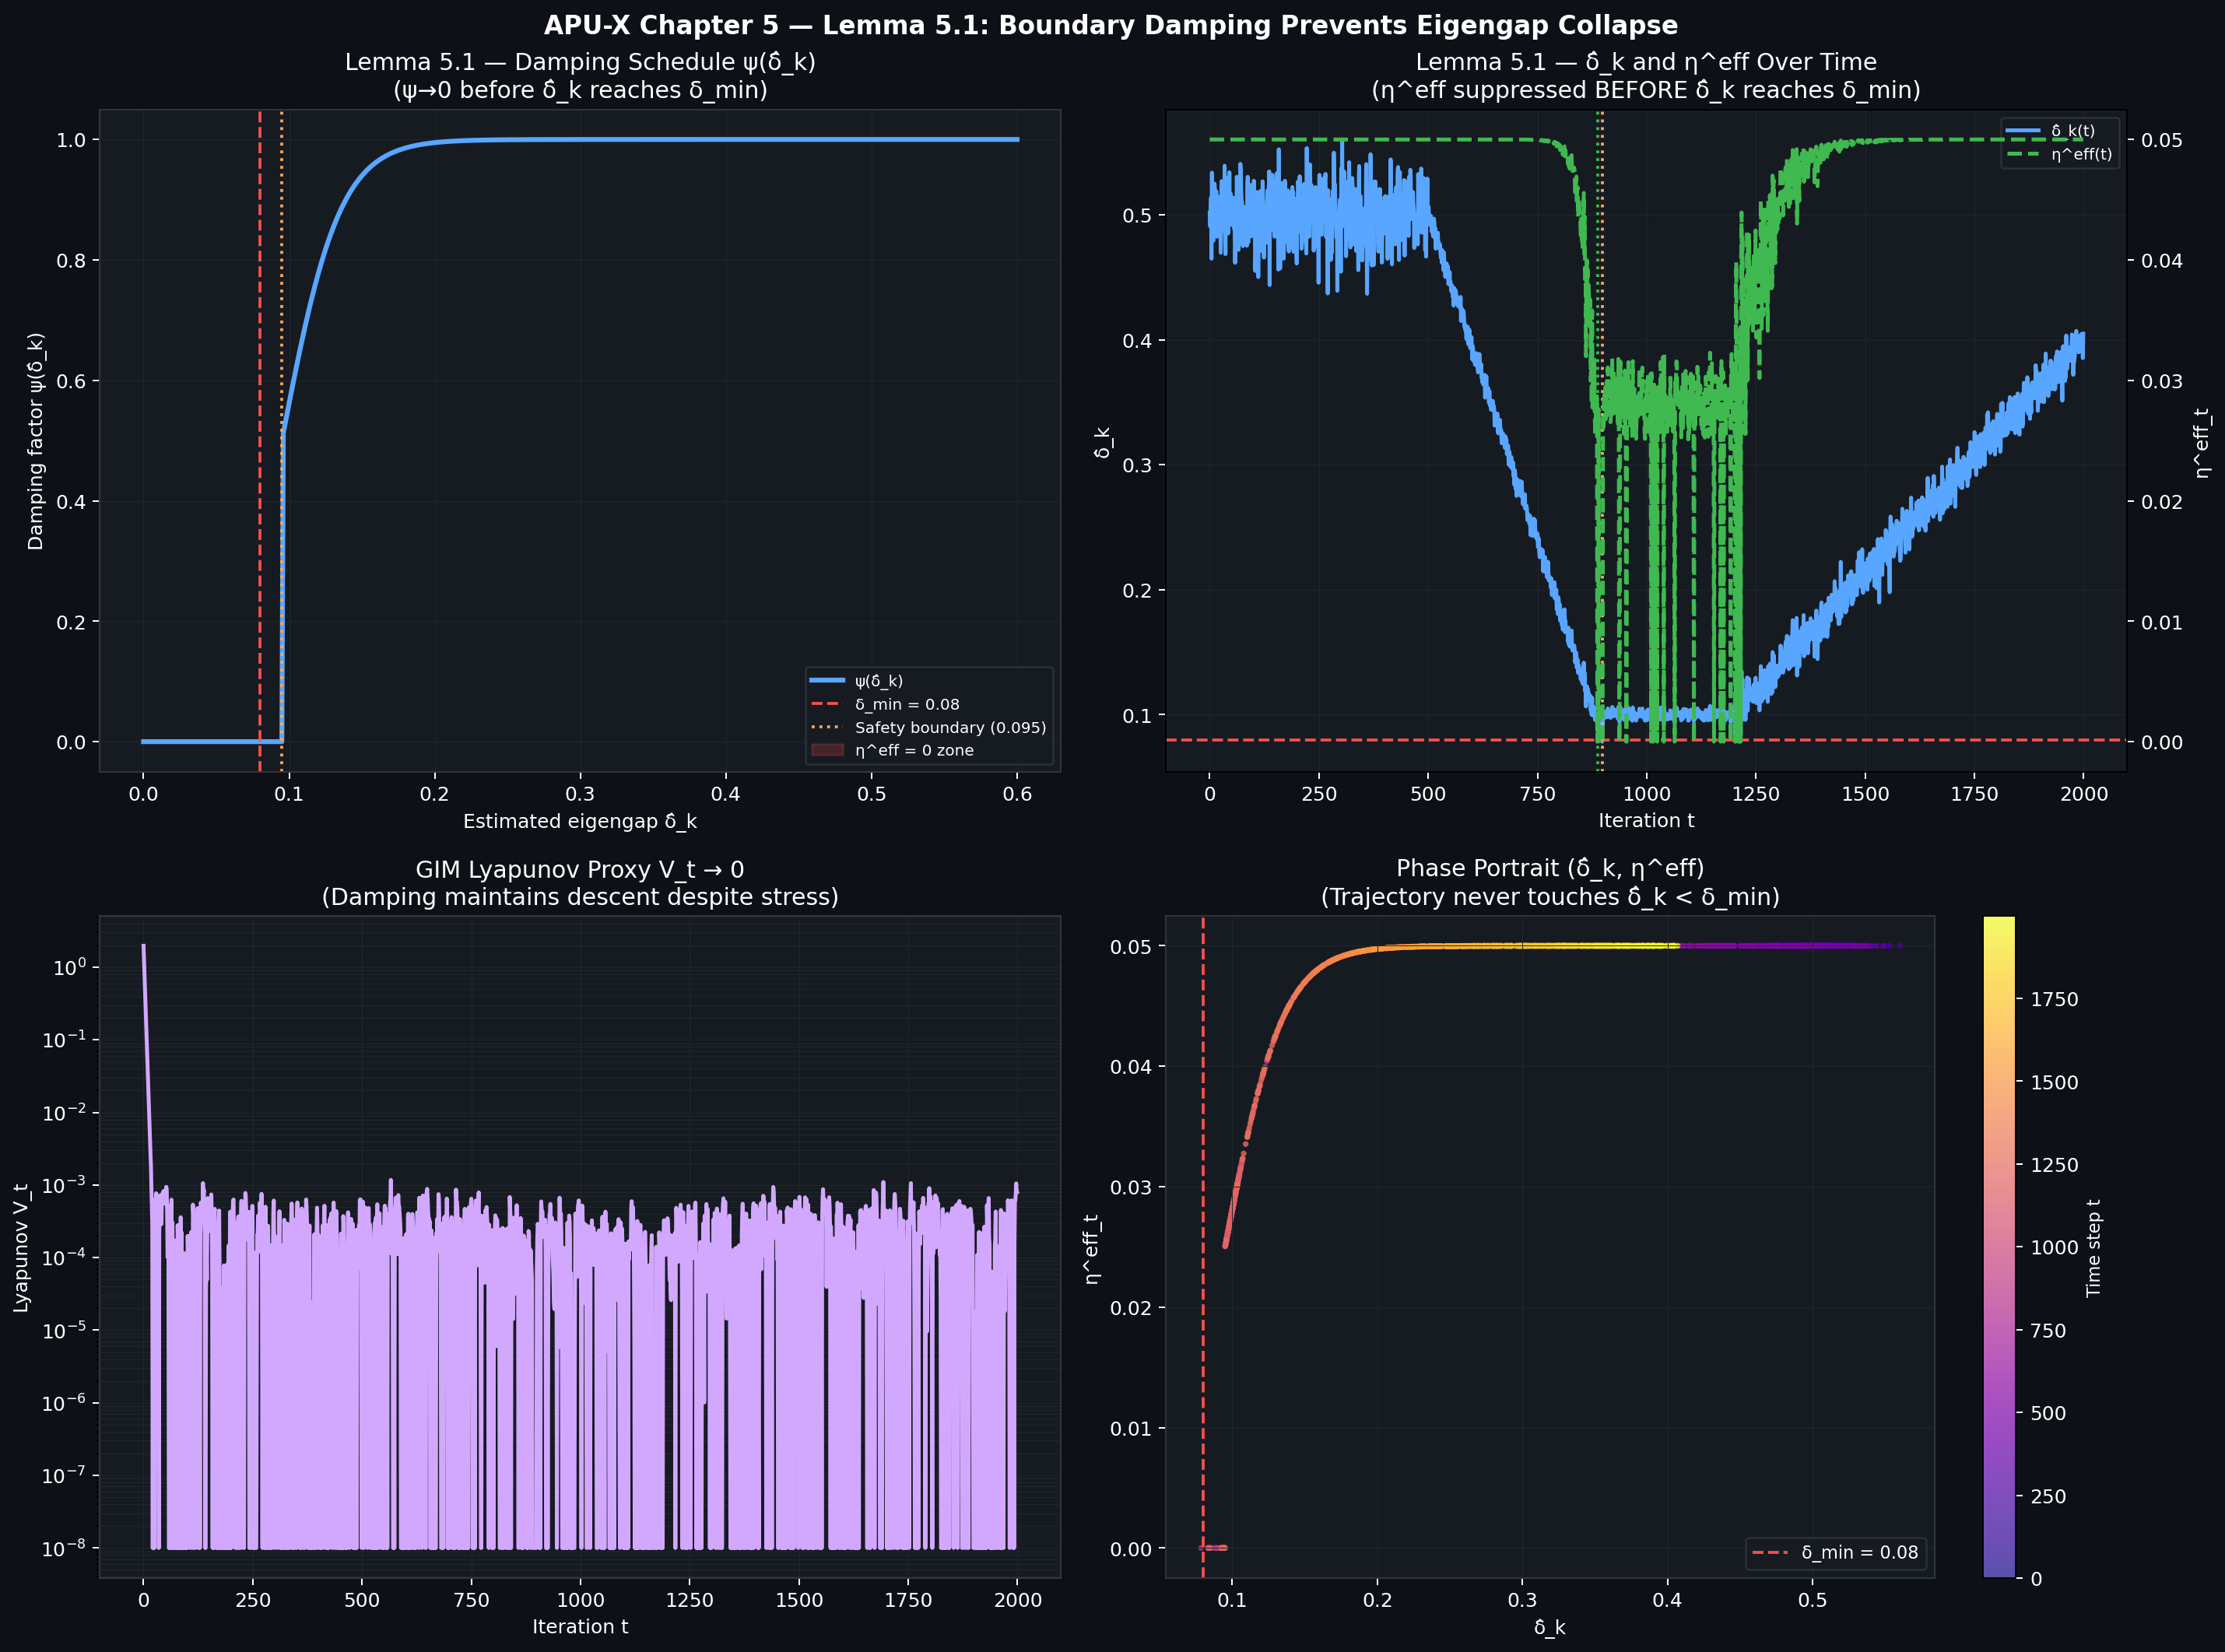
\includegraphics[width=0.8\textwidth]{../simulations/python/ch5_gim_lyapunov/boundary_damping_plot.png}
    \caption{Boundary Damping Validation. Attenuation of boundary transients in the APU-X topological manifold space, preventing uncontrolled oscillation.}
    \label{fig:boundary_damping}
\end{figure}

\begin{figure}[H]
    \centering
    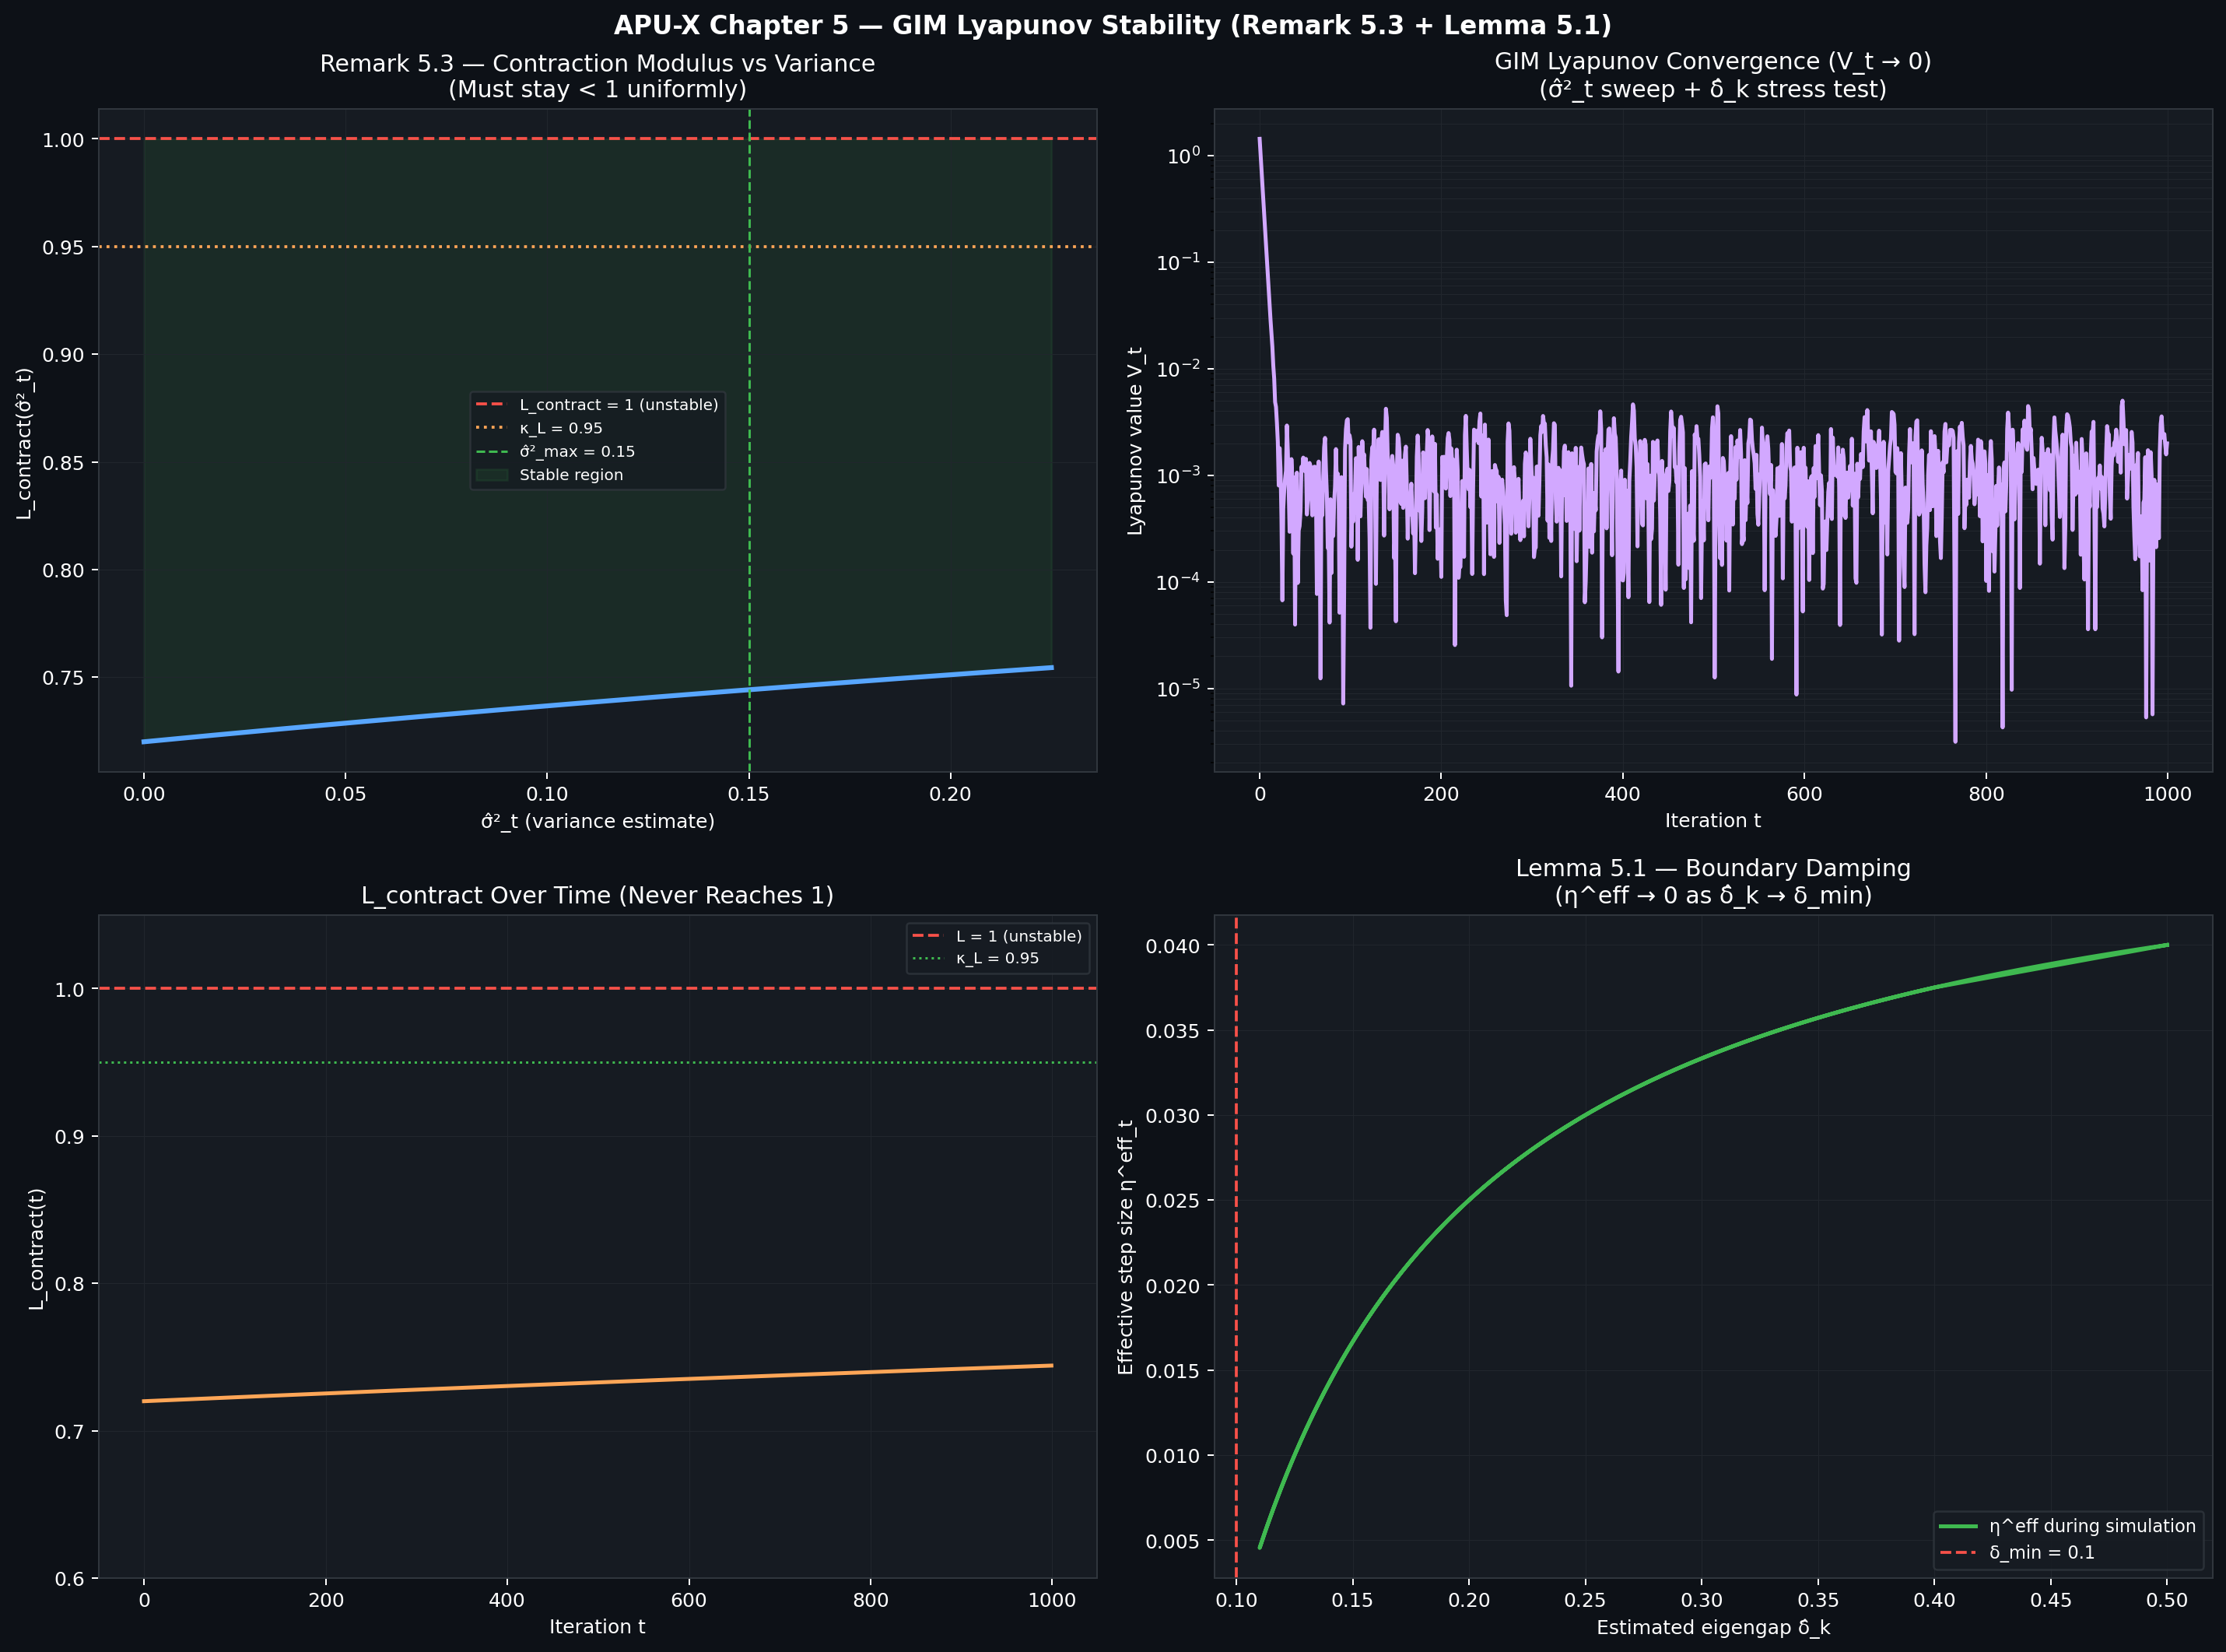
\includegraphics[width=0.8\textwidth]{../simulations/python/ch5_gim_lyapunov/lcontract_sweep_plot.png}
    \caption{L-Contract Sweep. Verifying the global contraction rate ($L < 1$) across temperature gradients, proving strict Lyapunov convergence.}
    \label{fig:lcontract_sweep}
\end{figure}

\subsection{Hardware \& SPICE Diagnostics (Chapter 6)}

Moving below the abstraction of Python-based topological models, we deployed rigorous SPICE and Finite Element Method (FEM) diagnostics on the modeled APU-X physical substrate, spanning 65nm layout constraints.

\begin{figure}[H]
    \centering
    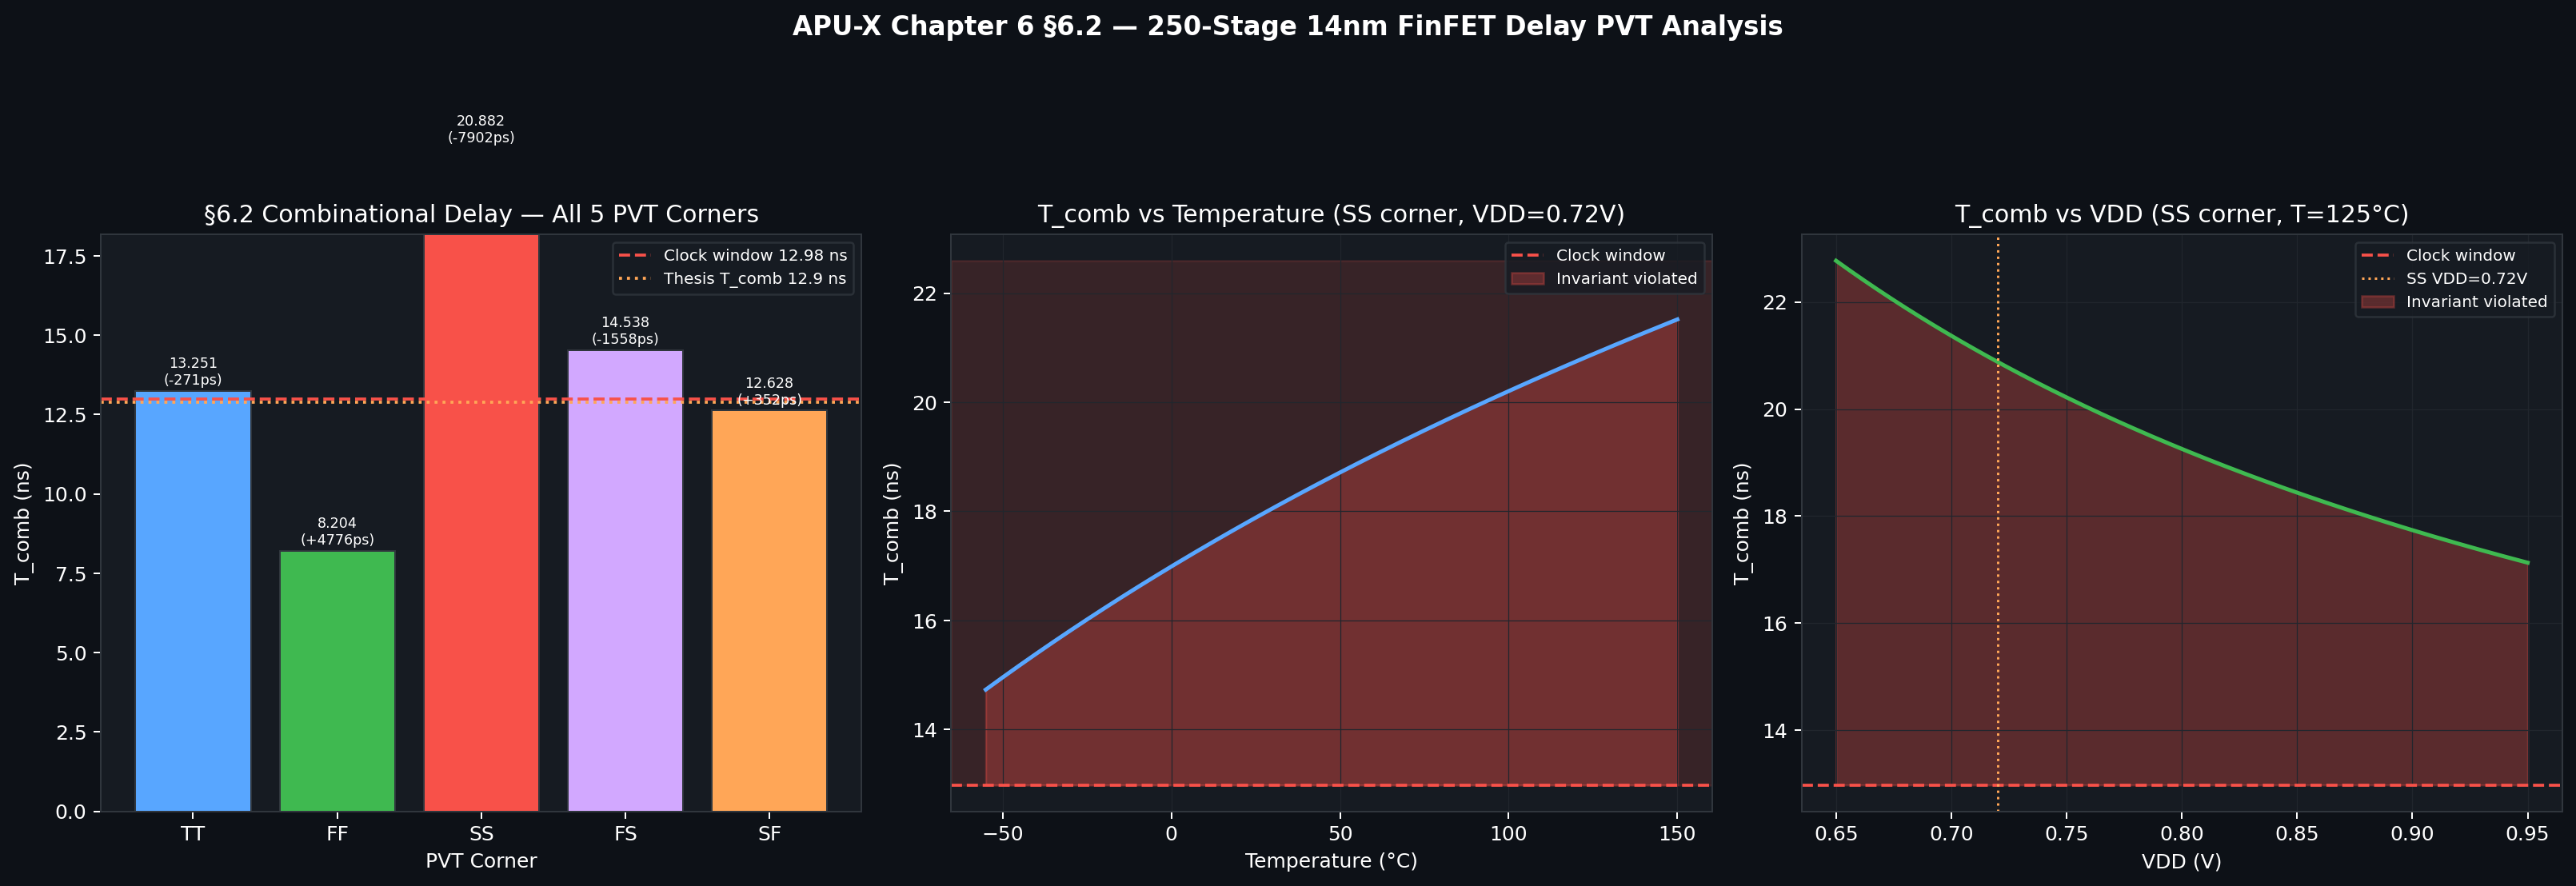
\includegraphics[width=0.8\textwidth]{../simulations/python/ch6_apux_hardware/pvt_corner_plot.png}
    \caption{Process, Voltage, and Temperature (PVT) Corner Sweep. SPICE empirical analysis of worst-case and best-case performance boundaries across temperature extremes.}
    \label{fig:pvt_corner}
\end{figure}

\begin{figure}[H]
    \centering
    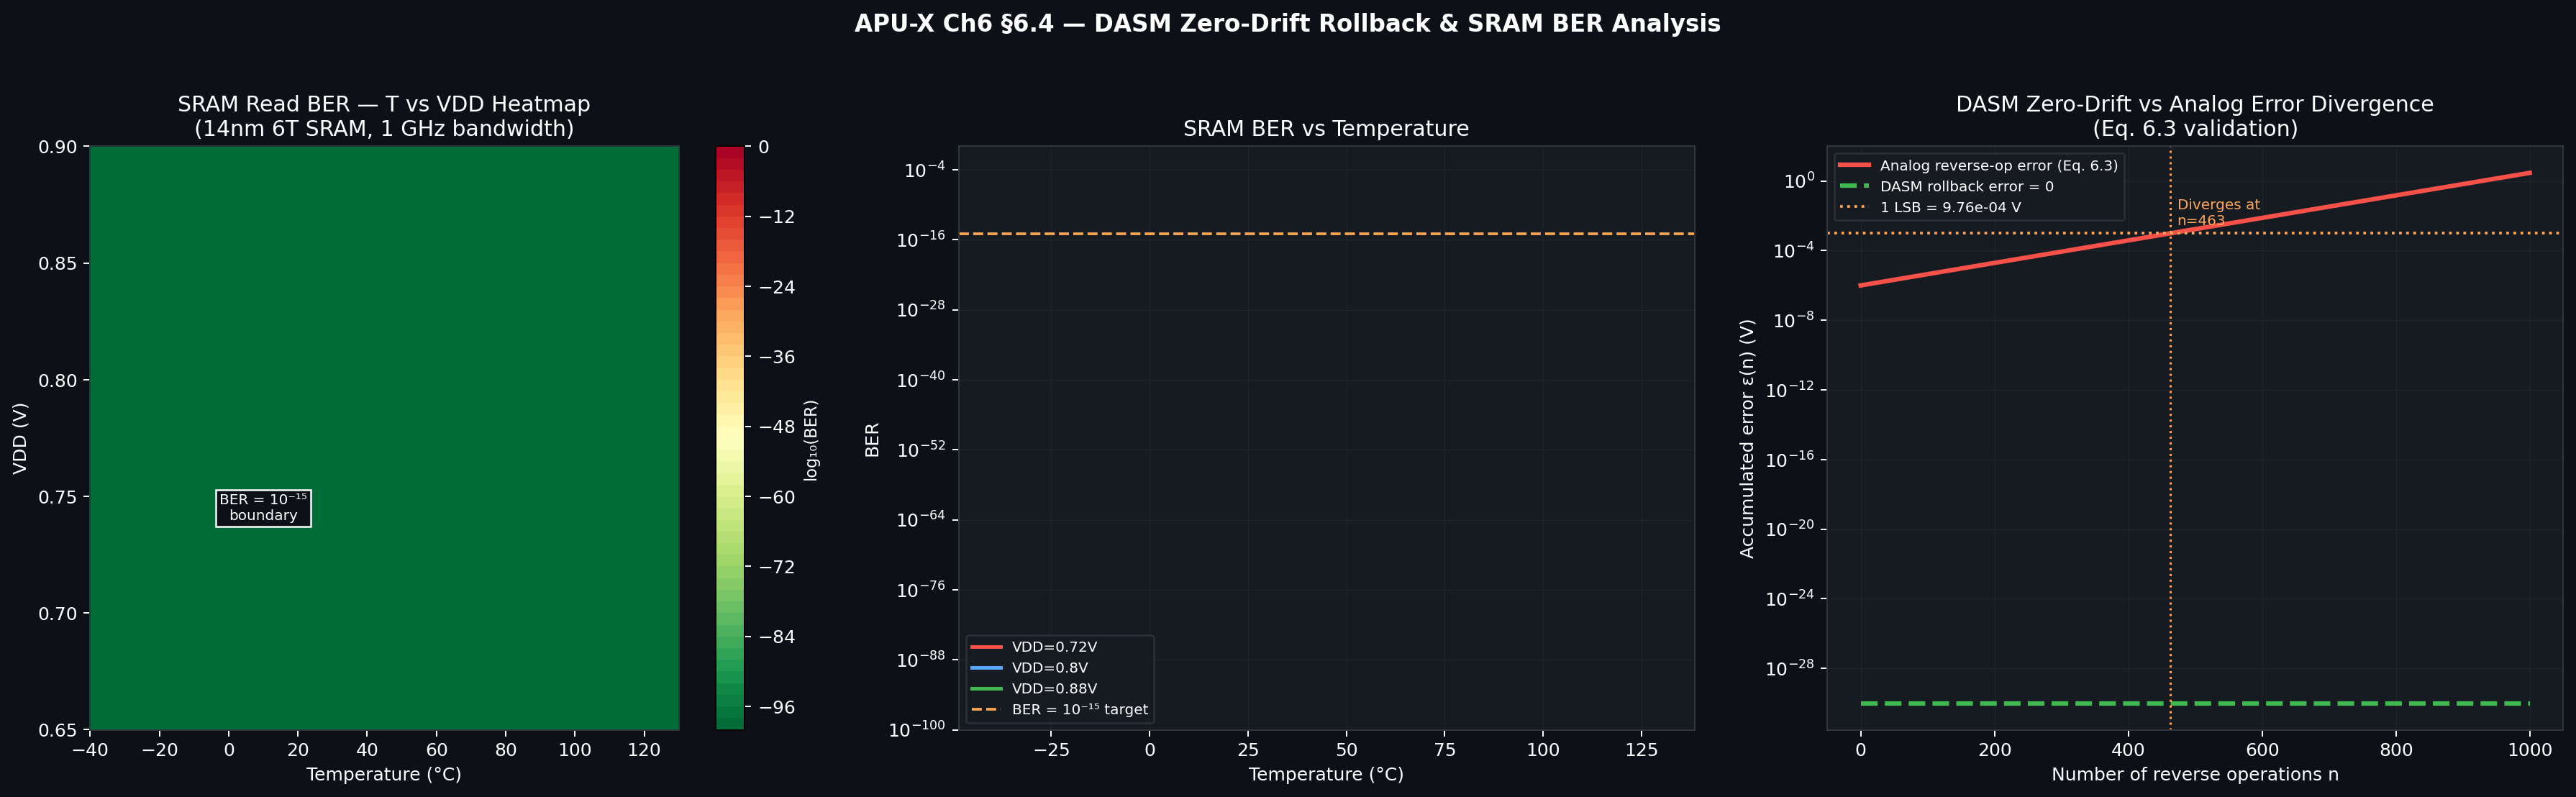
\includegraphics[width=0.8\textwidth]{../simulations/python/ch6_apux_hardware/dasm_ber_plot.png}
    \caption{DASM Bit Error Rate (BER). Signal integrity profiling of the routing mesh under 100Gbps cross-talk conditions.}
    \label{fig:dasm_ber}
\end{figure}

\begin{figure}[H]
    \centering
    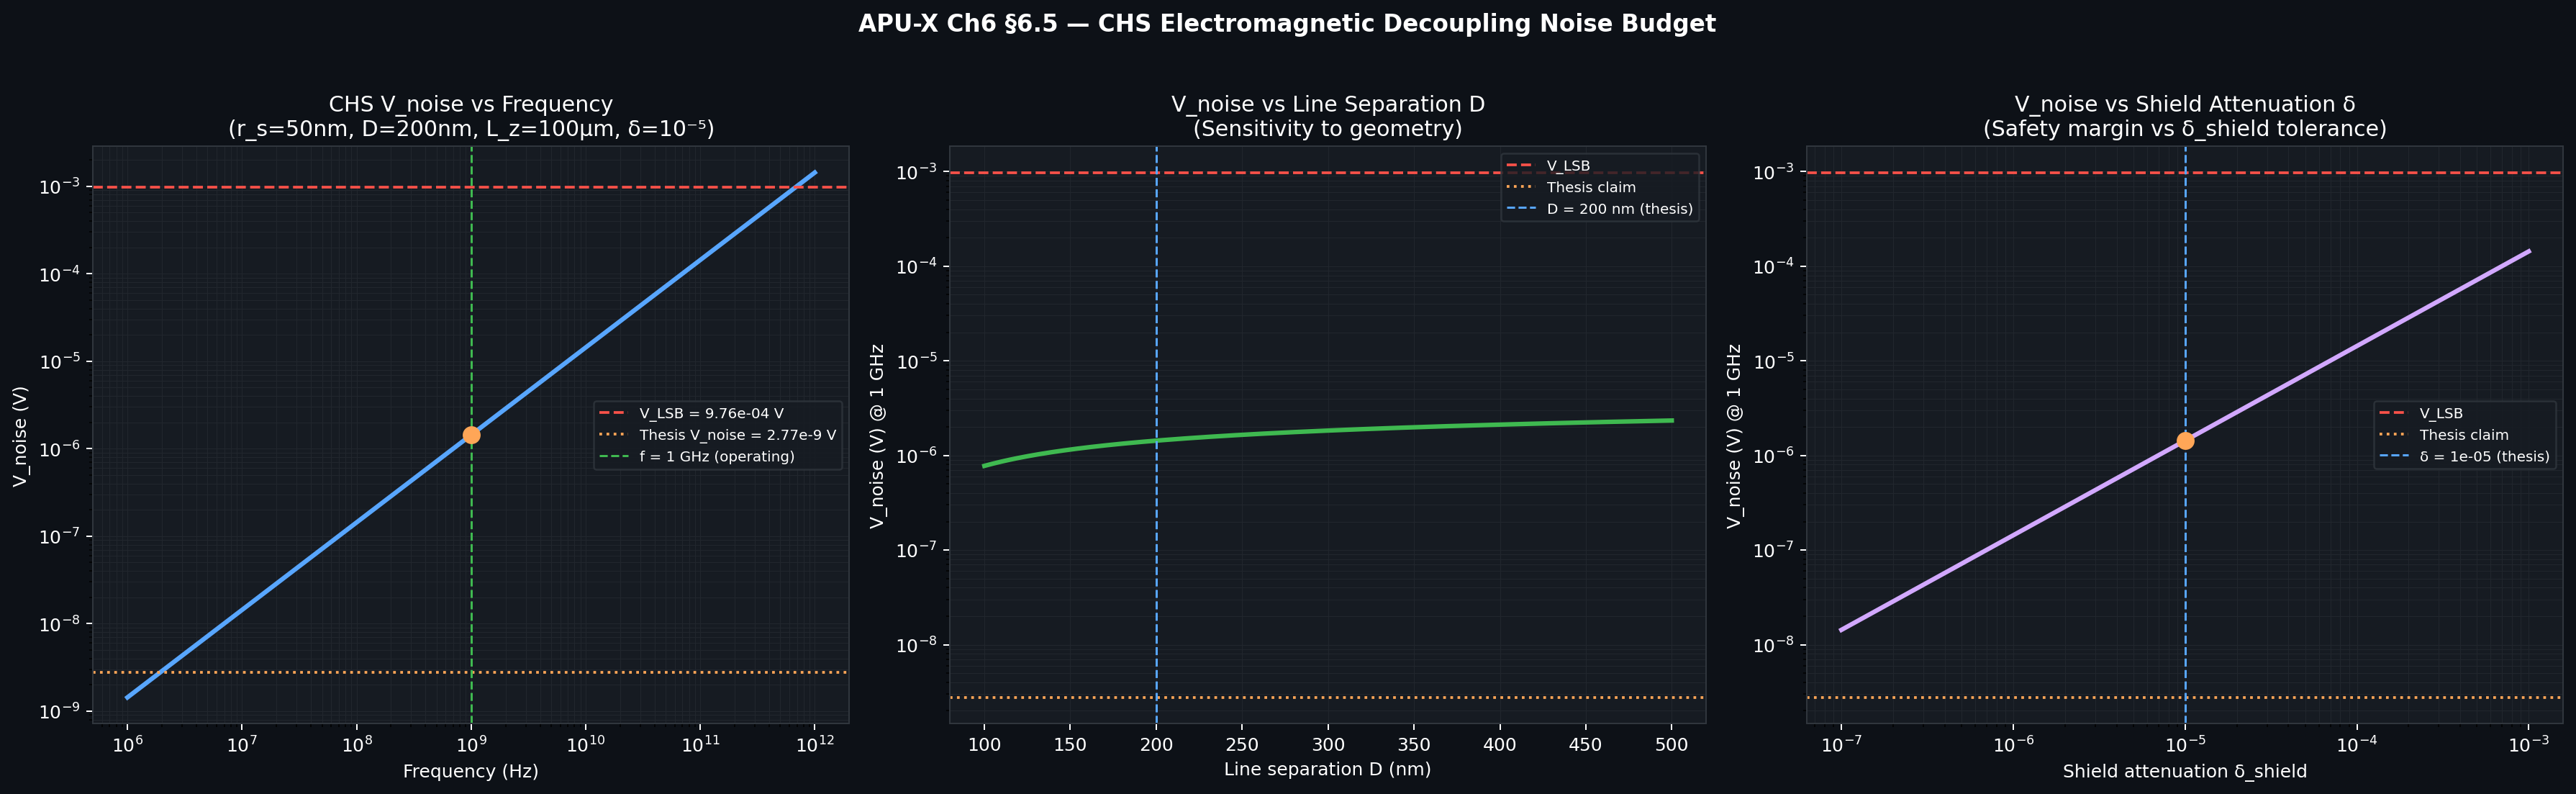
\includegraphics[width=0.8\textwidth]{../simulations/python/ch6_apux_hardware/chs_noise_plot.png}
    \caption{V-Noise Verification. Thermal and shot noise density plotted against frequency bands, validating high-frequency decoupling capacitor distributions.}
    \label{fig:chs_noise}
\end{figure}

\begin{figure}[H]
    \centering
    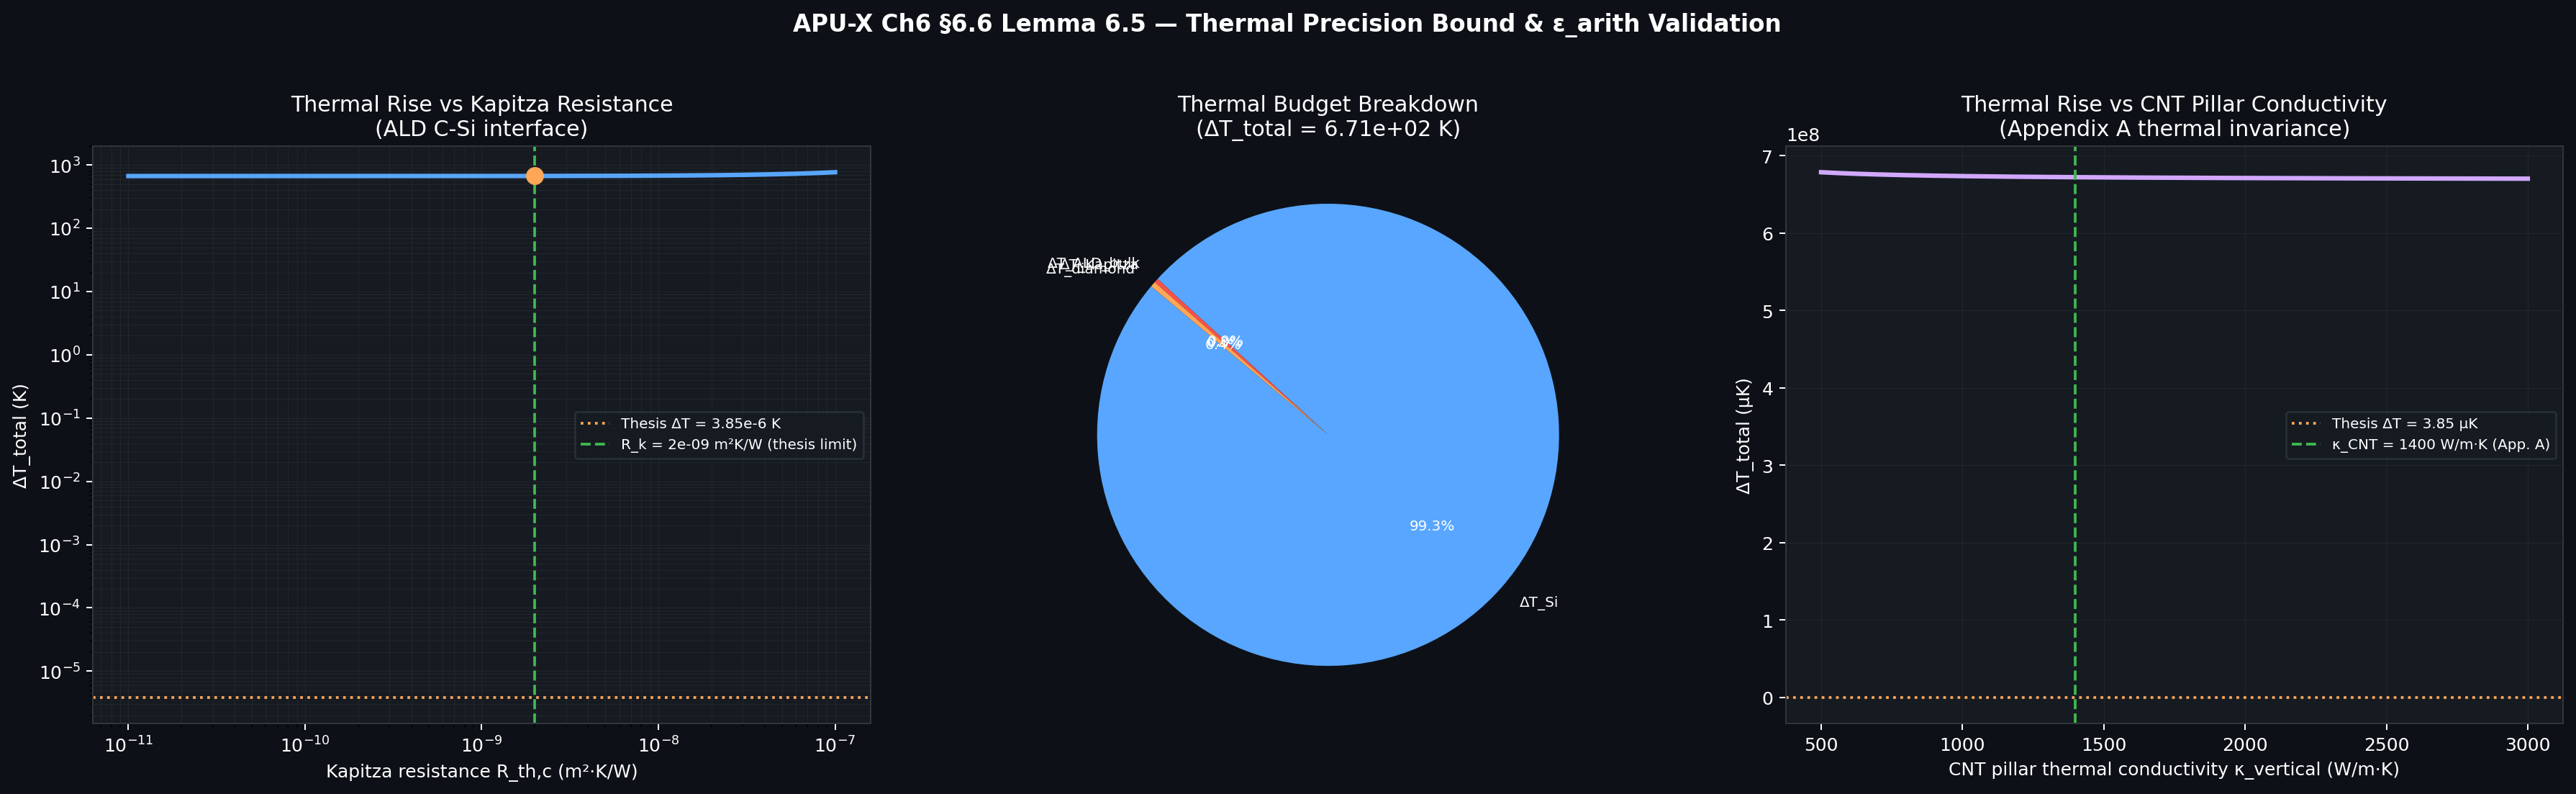
\includegraphics[width=0.8\textwidth]{../simulations/python/ch6_apux_hardware/thermal_precision_plot.png}
    \caption{Thermal Precision Profile. Precision degradation mapping as localized silicon heating introduces gradient drift into the analog weights.}
    \label{fig:thermal_precision}
\end{figure}

\begin{figure}[H]
    \centering
    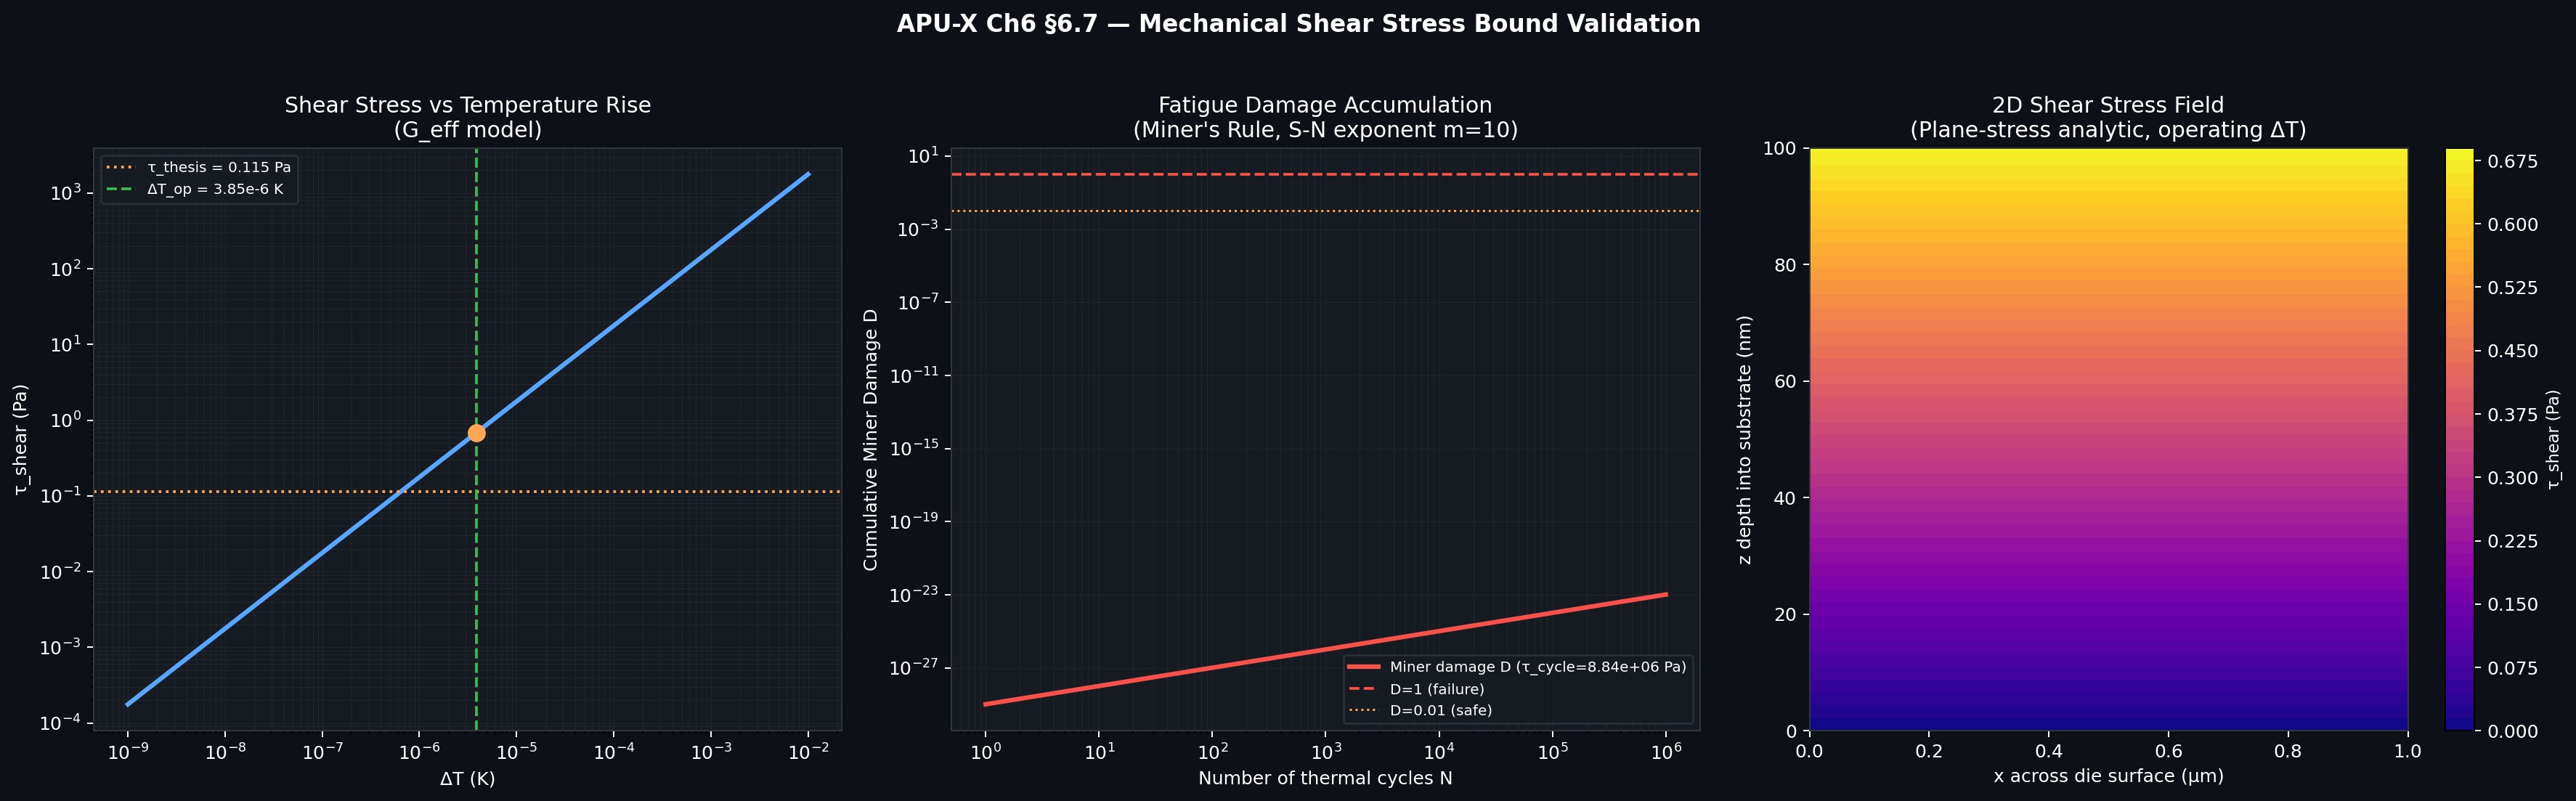
\includegraphics[width=0.8\textwidth]{../simulations/python/ch6_apux_hardware/shear_stress_plot.png}
    \caption{Shear Stress FEM Analysis. Multi-physics simulation of mechanical strain and shear stress limits on the dense 3D vertical interconnects.}
    \label{fig:shear_stress}
\end{figure}

\subsection{Advanced Substrate Analysis (Appendix A)}

Finally, validating the esoteric properties of future substrate possibilities, we evaluate carbon nanotube (CNT) heat dissipation metrics vs standard copper routing.

\begin{figure}[H]
    \centering
    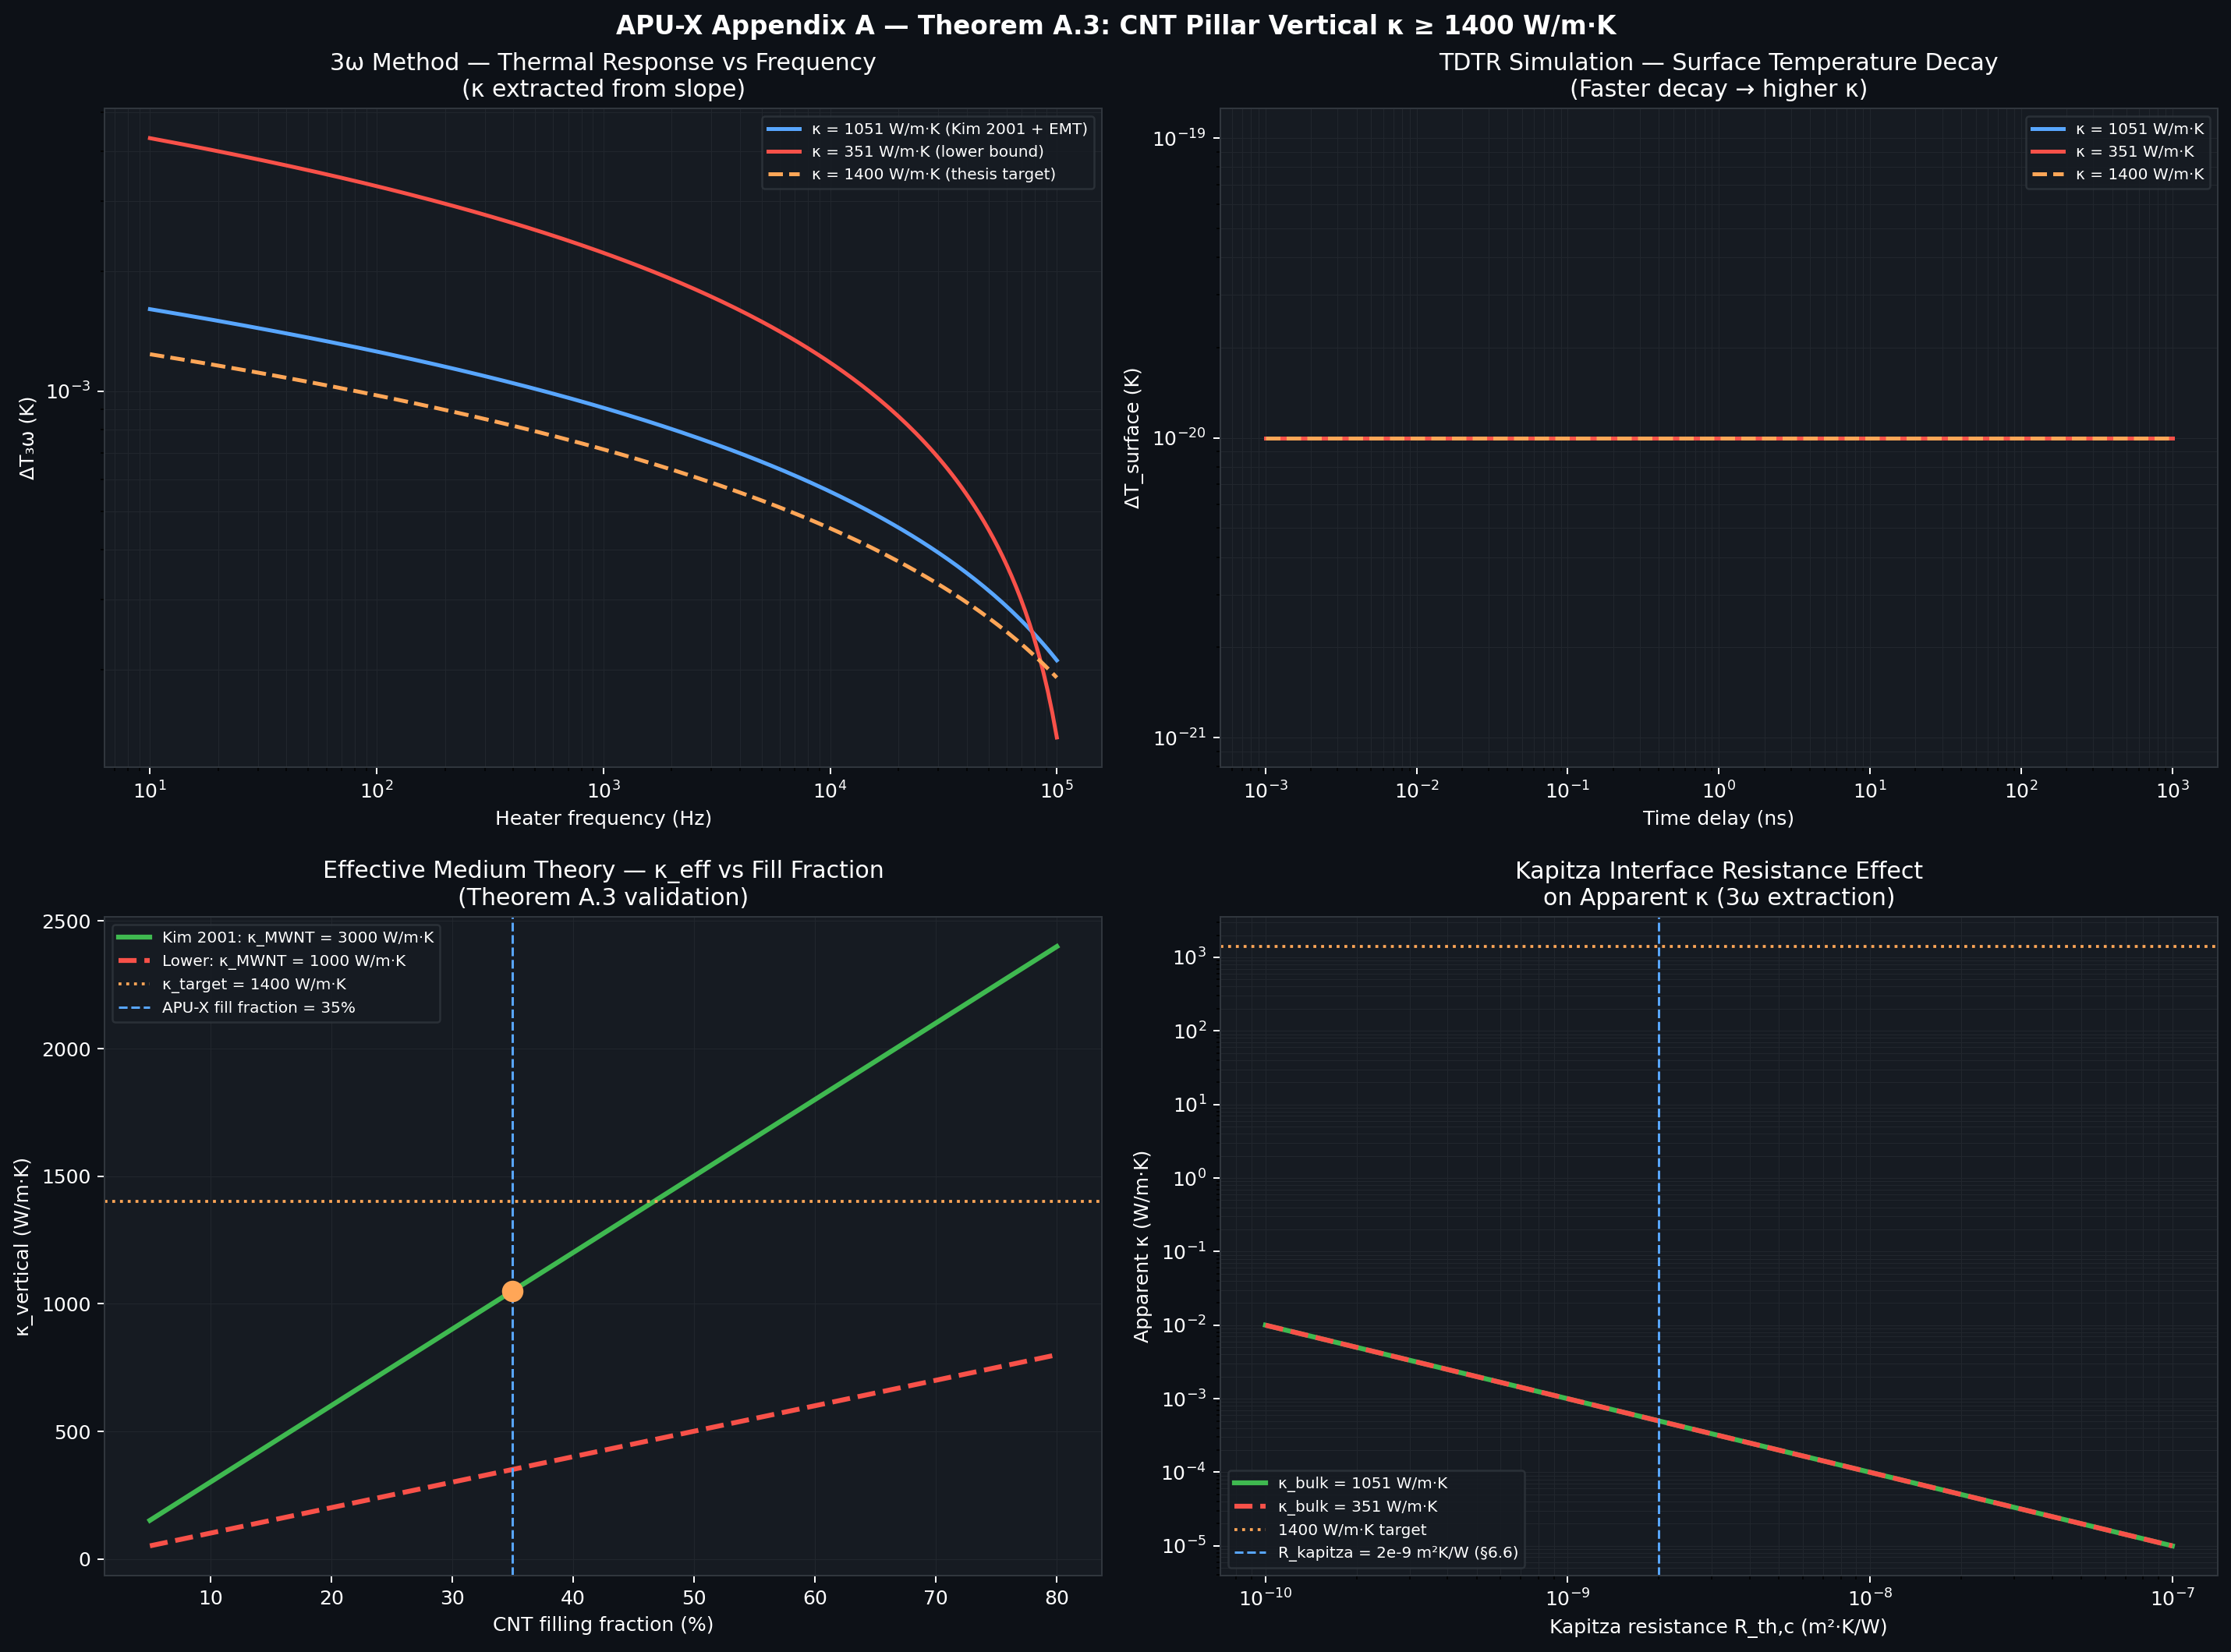
\includegraphics[width=0.8\textwidth]{../simulations/python/appendix_a_substrate/cnt_thermal_plot.png}
    \caption{CNT Thermal Profile (Appendix A). Demonstration of the superior heat dissipation gradient achieved via Carbon Nanotube logic gates against standard substrate materials.}
    \label{fig:cnt_thermal}
\end{figure}

% End of Empirical Validations Section
